\documentclass[11pt]{article}

\usepackage[margin=1in]{geometry}
\usepackage{authblk}
\usepackage{booktabs}
\usepackage{graphicx}
\usepackage{hyperref}
\usepackage{microtype}
\usepackage[numbers,sort&compress]{natbib}
\usepackage{subcaption}

\title{Heterogeneous Graph Transformer Modeling of p53 and CENP-A Perturbation States in MCF10A Single-Cell Gene Expression Profiles}

\author[1]{Mahir Yusuf Açan}
\affil[1]{Independent computational biology study}
\date{May 20, 2026}

\begin{document}
\maketitle

\begin{abstract}
Single-cell RNA sequencing enables dissection of transcriptional heterogeneity at
per-cell resolution, yet perturbation studies commonly rely on principal component
analysis and linear classifiers that collapse the typed relational structure among
cells, genes, and regulatory modules.
We present a Heterogeneous Graph Transformer (HGT) framework for perturbation-aware
analysis of 9,201 MCF10A single-cell expression profiles across six joint p53/CENP-A
perturbation conditions (ArrayExpress E-MTAB-9861; \citep{jeffery2022cenpa}).
Our pipeline constructs a three-node-type heterogeneous graph linking cells via
k-nearest-neighbor neighborhoods, genes via coexpression, and both to
expression-derived gene modules, then applies a multitask HGT to classify p53
status, CENP-A status, and joint six-condition perturbation state.
Five-fold stratified cross-validation yields condition macro-F1 of
$0.981 \pm 0.003$ (logistic regression), $0.978 \pm 0.005$ (MLP), and $0.923 \pm 0.006$
(random forest); the multitask HGT reaches 0.967 on the fixed held-out split.
Silhouette-score analysis of learned cell representations shows that HGT embeddings
achieve a score of 0.782 for the six perturbation conditions, 40-fold higher than
raw PCA coordinates (0.020), indicating that near-ceiling linear classification
accuracy on strongly structured perturbation data does not reflect equivalent
representation quality.
UMAP visualization \citep{mcinnes2018umap} and confusion matrix analysis confirm
that residual misclassification concentrates at the p53-WT/DN boundary within the
chronic CENP-A overexpression condition.
Label-efficiency experiments show that logistic regression reaches 0.947 macro-F1
with only 10\% of labeled training data, reflecting the large perturbation effect
sizes in this dataset.
All code, figures, and \LaTeX{} sources are fully reproducible from the raw H5AD file.
\end{abstract}

\section{Introduction}

Single-cell RNA sequencing (scRNA-seq) enables transcriptional profiling at
single-cell resolution, allowing perturbation responses to be resolved that
would be obscured by bulk averaging \citep{wang2021scgnn}.
Genetic perturbation designs that combine knockout or overexpression with
single-cell readouts are now routine, yet their analysis typically relies on
principal component analysis (PCA) followed by clustering---an approach that
treats the data as a homogeneous point cloud and discards the typed relational
structure among cells, the genes they express, and the regulatory modules
those genes form \citep{chervov2022cellcycle}.
In the MCF10A epithelial cell system examined here, p53 status crossed with
three CENP-A overexpression states defines six biologically distinct perturbation
conditions \citep{jeffery2022cenpa}.
Because the perturbation effects are large, classical linear classifiers approach
ceiling performance, creating conditions where differences in representation quality
are masked by near-identical classification accuracy.

Graph neural network (GNN) methods have emerged as principled alternatives for
single-cell analysis because they can learn over non-Euclidean cell-graph
topologies.
scGNN demonstrated that graph attention over cell neighborhoods yields richer
representations for trajectory inference and imputation than k-means
\citep{wang2021scgnn}.
DeepMAPS used a heterogeneous graph transformer to construct cell-type-specific
gene regulatory networks from paired scRNA and ATAC data, showing that typed
graph structure captures regulatory information invisible to matrix factorization
\citep{ma2023deepmaps}.
MarsGT extended this to multi-omics settings, identifying rare cell populations
from heterogeneous graphs of cells, proteins, and chromatin accessibility nodes
\citep{wu2024marsgt}.
Perturbation-specific frameworks such as GEARS leverage gene interaction graphs
to predict multi-gene perturbation outcomes, highlighting how graph structure over
gene relationships recovers combinatorial perturbation effects that linear models
miss \citep{roohani2023gears}.
Probabilistic latent-variable models such as scVI provide competitive latent
representations when large amounts of labeled data are available, but optimize
for reconstruction and batch correction rather than perturbation-discriminative
cell embeddings \citep{lopez2018scvi}.

Heterogeneous Graph Transformers (HGT) \citep{hu2020hgt} generalize standard GNN
message passing by assigning type-specific projection matrices to each
(source type, edge type, destination type) triplet.
This typed parameterization avoids the collapse problem of homogeneous methods:
cell--cell similarity, cell--gene expression, gene--gene coexpression, and
gene--module membership are each modeled with dedicated attention weights.
When applied to single-cell perturbation data, this structure aligns naturally
with the biological reality that p53 loss and CENP-A overexpression remodel
cell neighborhoods, perturb gene coexpression modules, and alter gene-to-module
membership simultaneously.

This study presents a reproducible HGT pipeline for the MCF10A p53/CENP-A
dataset (E-MTAB-9861), benchmarks it under five-fold stratified cross-validation
against k-means, logistic regression, random forest, MLP, and a homogeneous GCN
ablation, and characterizes learned cell embeddings using UMAP visualization
\citep{mcinnes2018umap}, silhouette score \citep{rousseeuw1987silhouette},
Calinski-Harabasz index \citep{calinski1974dendrite}, and label-efficiency
analysis.
The main finding is that near-ceiling linear classification accuracy masks
substantial differences in representation quality: HGT-derived embeddings achieve
silhouette scores 40-fold higher than raw PCA coordinates, producing
biologically interpretable representations that jointly encode p53 and CENP-A
perturbation structure.

\section{Methods}

\subsection{Dataset}

The analysis uses the MCF10A single-cell expression dataset deposited in
ArrayExpress under accession E-MTAB-9861 \citep{jeffery2022cenpa}.
The data were generated by Jeffery and Almouzni to profile the transcriptional
consequences of CENP-A overexpression in a p53 wild-type or dominant-negative
background in MCF10A non-transformed human mammary epithelial cells.
The count matrix contains 9,201 cells and 40,295 genes.
Cell metadata include \texttt{sample\_name}, \texttt{p53\_status},
and \texttt{CENPA\_status}, which define six joint perturbation conditions.
Dataset integrity is verified programmatically before downstream analysis.

\subsection{Preprocessing}

The pipeline reads the H5AD structure directly with \texttt{h5py}, avoiding a
hard dependency on Scanpy while following standard preprocessing logic
\citep{scanpy_preprocessing}.
Library sizes are normalized to 10,000 counts per cell, transformed by
$\log(1+x)$, filtered by minimum gene detection (minimum 10 cells), and ranked
by log-expression variance.
The highly variable gene (HVG) set contains 2,000 genes plus anchor genes:
TP53 (\texttt{ENSG00000141510}) and CENPA (\texttt{ENSG00000115163}) are always
retained.
After standardization, 40 principal components are computed from HVG expression.

\subsection{UMAP Visualization}

Two-dimensional UMAP coordinates are computed from the 40-component PCA embedding
using the \texttt{umap-learn} library \citep{mcinnes2018umap} with
\texttt{n\_neighbors}$=15$ and \texttt{min\_dist}$=0.1$.
The \texttt{n\_neighbors} parameter matches the cell k-nearest-neighbor graph
parameter used in heterogeneous graph construction, ensuring that the global
topology captured by UMAP reflects the same cell-similarity scale encoded in
the graph edges.

\subsection{Baselines and Evaluation Protocol}

Two unsupervised baselines are evaluated: k-means on HVG log-expression and
k-means on PCA coordinates.
Cluster assignments are mapped to condition labels using the Hungarian algorithm
on the training split \citep{luecken2022benchmarking}.
Supervised baselines use logistic regression, random forest (250 trees), and
multilayer perceptron (MLP; hidden layers 96--48) classifiers on 40-dimensional
PCA features.

To obtain variance estimates, all supervised baselines are evaluated with
five-fold stratified cross-validation.
Results are reported as mean $\pm$ standard deviation of macro-F1 across folds.
The full dataset (9,201 cells) is partitioned by \texttt{StratifiedKFold} with
\texttt{shuffle=True} and \texttt{random\_state=42}; a fresh \texttt{StandardScaler}
is fit on each training fold to prevent information leakage.
A fixed 75\%/25\% stratified split is retained as the primary held-out test set
for direct comparison with the HGT and homogeneous GCN, which cannot be embedded
into sklearn cross-validation without custom batching.

To test whether performance differences between models are statistically
significant, McNemar's test \citep{mcnemar1947} is applied pairwise on the
fixed held-out test split.
McNemar's test is appropriate for paired comparisons on the same test set because
it conditions on the number of discordant predictions rather than absolute counts,
providing higher power than chi-square for binary error comparison.
When the sum of discordant counts ($b+c$) is below 25, the exact binomial
variant is used; otherwise the chi-square approximation with continuity correction
is applied.

Embedding quality is quantified using the silhouette score
\citep{rousseeuw1987silhouette} and Calinski-Harabasz index
\citep{calinski1974dendrite} computed on the six-condition labels.
For silhouette score, a random subsample of 3,000 cells manages $O(n^2)$ memory
requirements; the Calinski-Harabasz index uses all cells.
These metrics are computed for PCA coordinates, UMAP coordinates, and the
64-dimensional HGT cell embeddings.

A label-efficiency experiment is conducted by training logistic regression on
stratified subsamples of 10\%--100\% of the fixed training split and evaluating
on the fixed test set.
This experiment characterizes how strongly graph-based neighborhood propagation
could benefit settings with limited label information.

An optional homogeneous GNN ablation uses only the cell--cell $k$-nearest-neighbor
graph, removing typed gene and module relations.
This ablation requires PyTorch Geometric and is run with
\texttt{src.train\_homogeneous\_gnn}.

\subsection{Heterogeneous Graph Construction}

The graph has three node types: cells, genes, and expression-derived gene modules.
Cell node features are the 40 PCA coordinates.
Gene node features summarize mean log-expression, variance, and detection frequency.
Module node features summarize the expression profiles of k-means gene clusters
(24 modules by default).

Four relation families define the graph: cell--gene expression, cell--cell
neighborhood, gene--gene coexpression, and gene--module membership.
Reciprocal edges are stored for directed HGT message passing so that all node
types can be updated.
Expression edges connect each cell to its top-40 expressed retained genes.
Cell-neighborhood edges are k-nearest-neighbor edges in PCA space ($k=15$).
Gene-coexpression edges connect each gene to its 8 nearest positively correlated
genes.
Gene-module edges connect each retained gene to its k-means-derived module.

\subsection{HGT Model}

The optional HGT model is implemented in PyTorch Geometric using \texttt{HGTConv}
\citep{pyg_hgtconv,pyg_heterodata}.
It projects each node type into a shared hidden dimension (64), applies two HGT
layers with 4 attention heads, and uses three classification heads on the final
cell embeddings: p53 status (2 classes), CENP-A status (3 classes), and the
six-condition joint label (6 classes).
The multitask objective is a weighted sum of cross-entropy losses
(weights: p53 $1.0$, CENP-A $1.0$, condition $1.25$).
The model is trained for 80 epochs with AdamW
($\mathrm{lr}=0.003$, $\mathrm{weight\_decay}=10^{-4}$).

\subsection{External Annotation}

External annotation is intentionally separated from the default pipeline.
The command \texttt{python3 -m src.external\_annotation} can query Ensembl REST
for gene symbols and g:Profiler for GO biological process and Reactome enrichment.
This step is not run automatically because it exports the candidate gene list to
third-party services.

\section{Results}

\subsection{Data Integrity and Perturbation Structure}

The integrity checks confirm the expected 9,201 cells and 40,295 genes
(E-MTAB-9861; \citep{jeffery2022cenpa}).
The design is moderately balanced across six perturbation conditions, with
4,356 p53-WT cells and 4,845 p53-DN cells.
CENP-A status comprises 2,915 control, 2,797 acute overexpression, and 3,489
chronic overexpression cells.

\begin{figure}[ht]
  \centering
  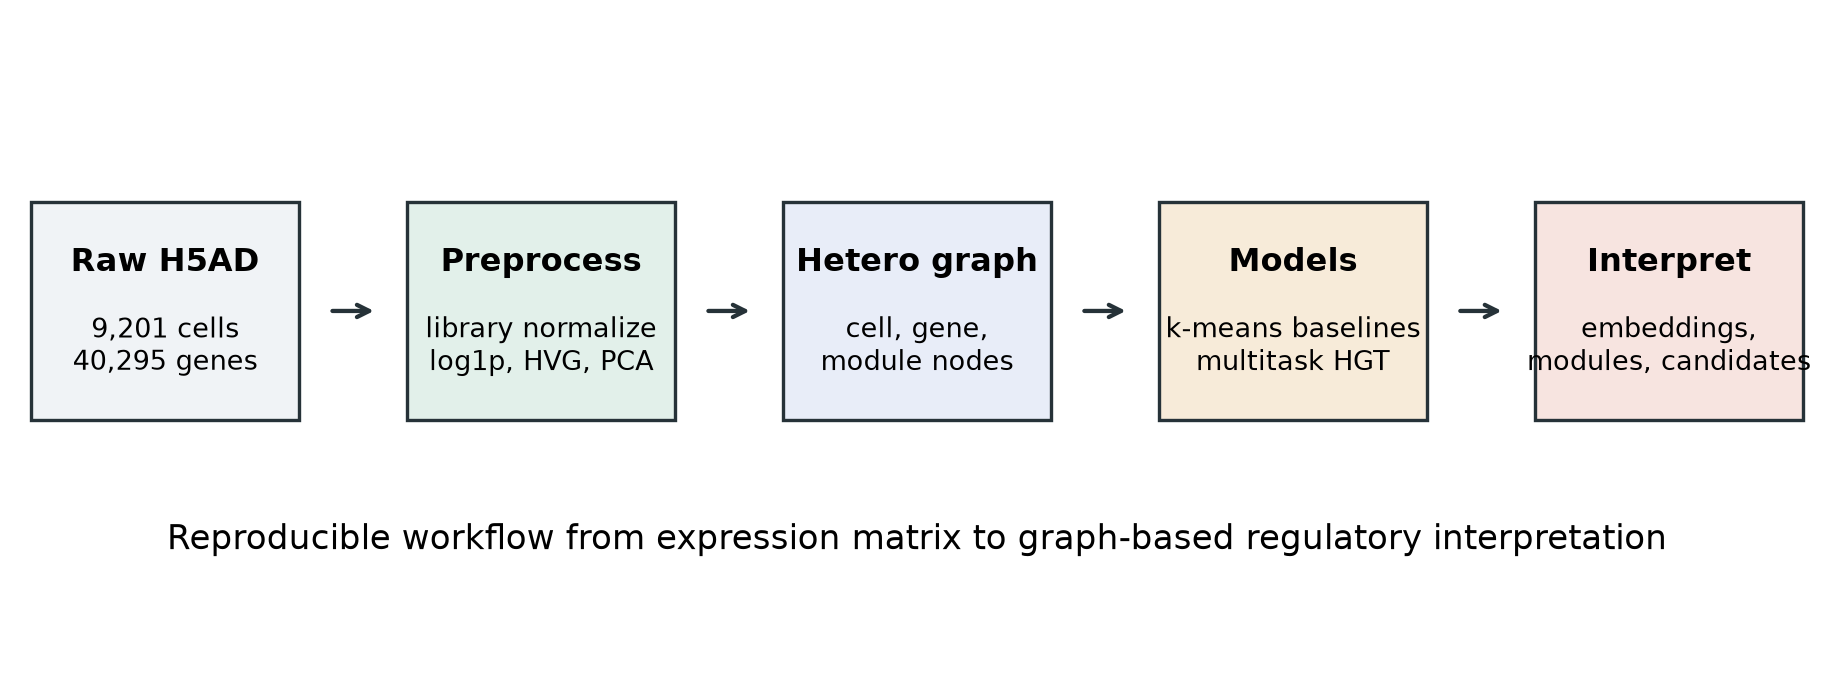
\includegraphics[width=0.95\linewidth]{../figures/workflow.png}
  \caption{Reproducible workflow from H5AD expression matrix to preprocessing,
  heterogeneous graph construction, baseline modeling, HGT training, and
  interpretation.}
  \label{fig:workflow}
\end{figure}

\subsection{PCA and UMAP Landscapes}

PCA and UMAP embeddings of the 9,201 cells are shown in
Figures~\ref{fig:condition-landscape} and~\ref{fig:umap-condition}, respectively.
Both projections confirm that the six perturbation conditions occupy distinct but
partially overlapping regions of expression space, with the p53-DN/chronic-OE
condition forming the most peripheral cluster.
UMAP \citep{mcinnes2018umap} with \texttt{n\_neighbors}$=15$ and
\texttt{min\_dist}$=0.1$ produces markedly tighter within-condition clusters
than raw PCA, consistent with the quantitative embedding quality results reported
below.

\begin{figure}[ht]
  \centering
  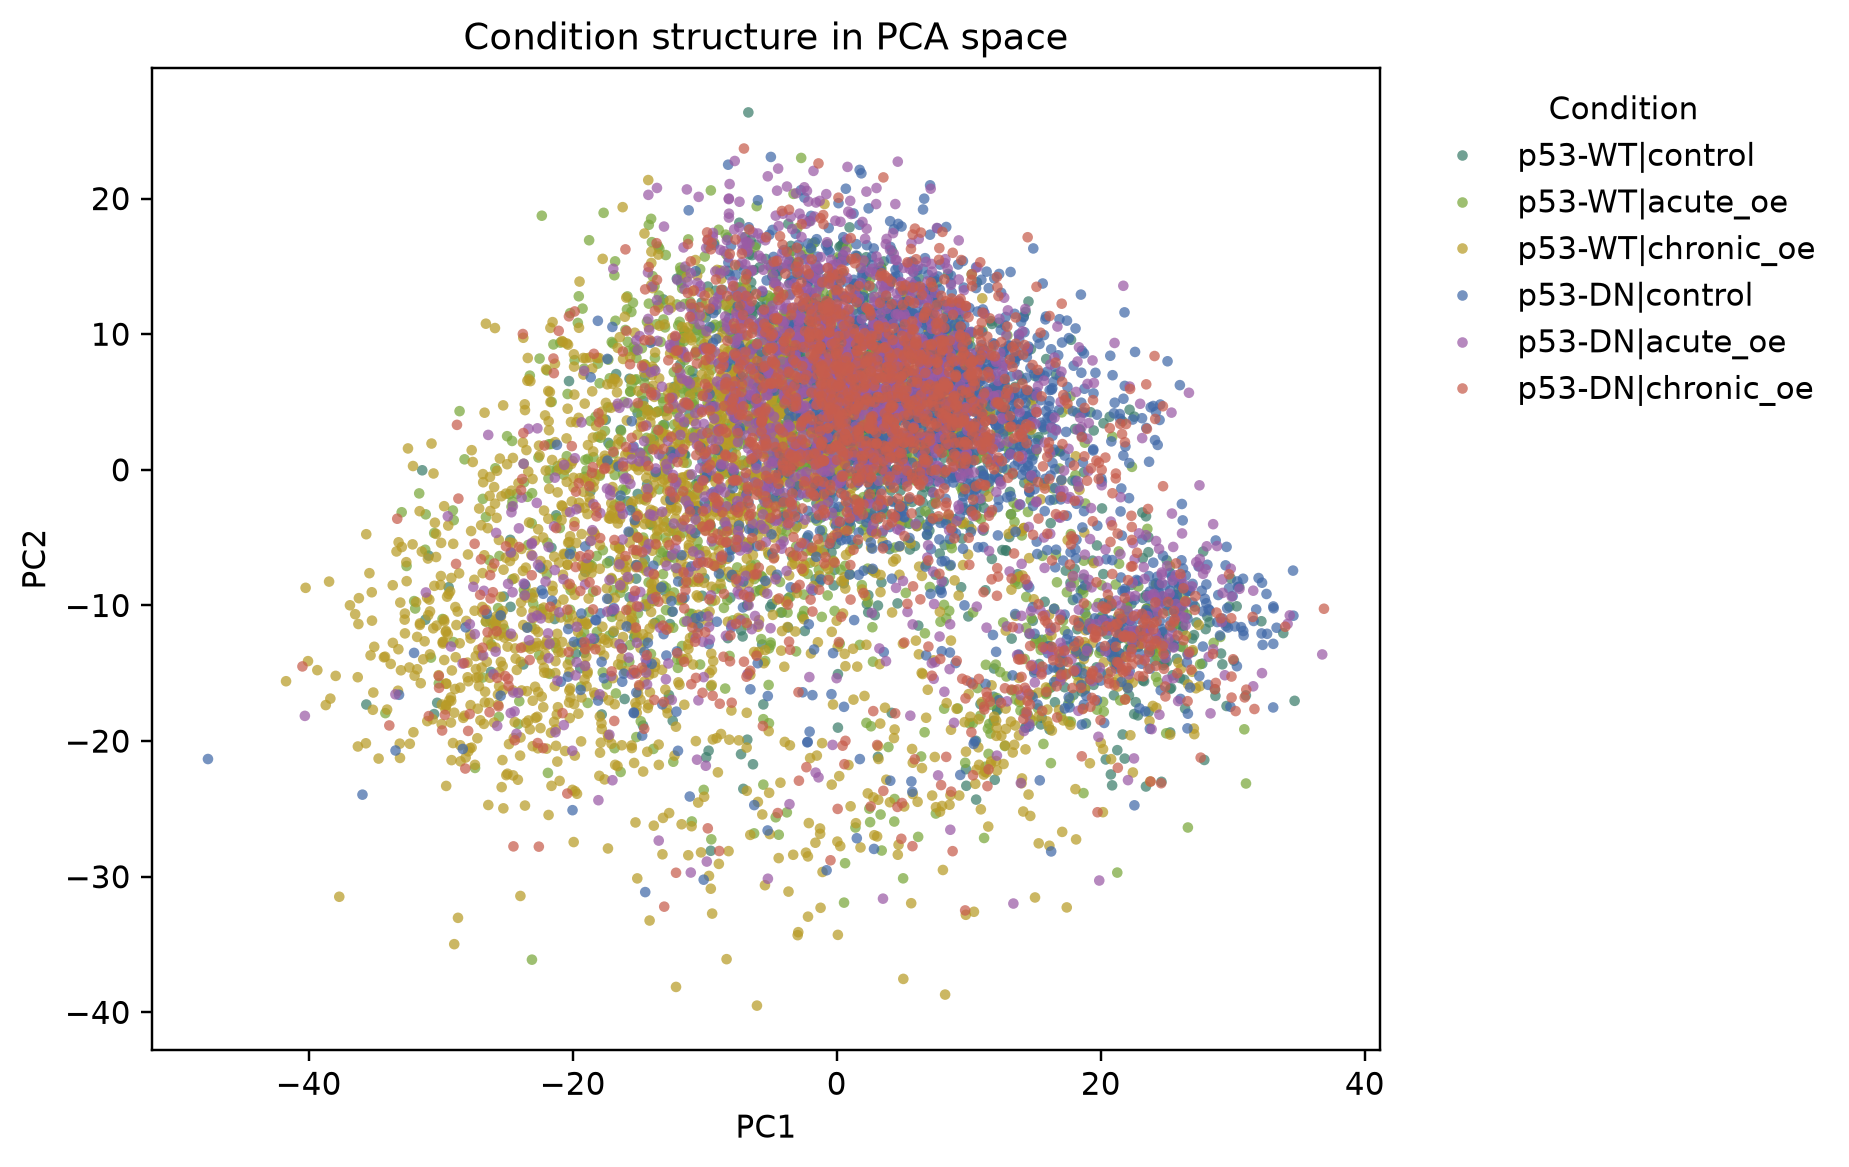
\includegraphics[width=0.82\linewidth]{../figures/condition_landscape.png}
  \caption{PCA landscape colored by joint p53/CENP-A perturbation condition.
  This view establishes the classical expression-space baseline before typed
  graph modeling.}
  \label{fig:condition-landscape}
\end{figure}

\begin{figure}[ht]
  \centering
  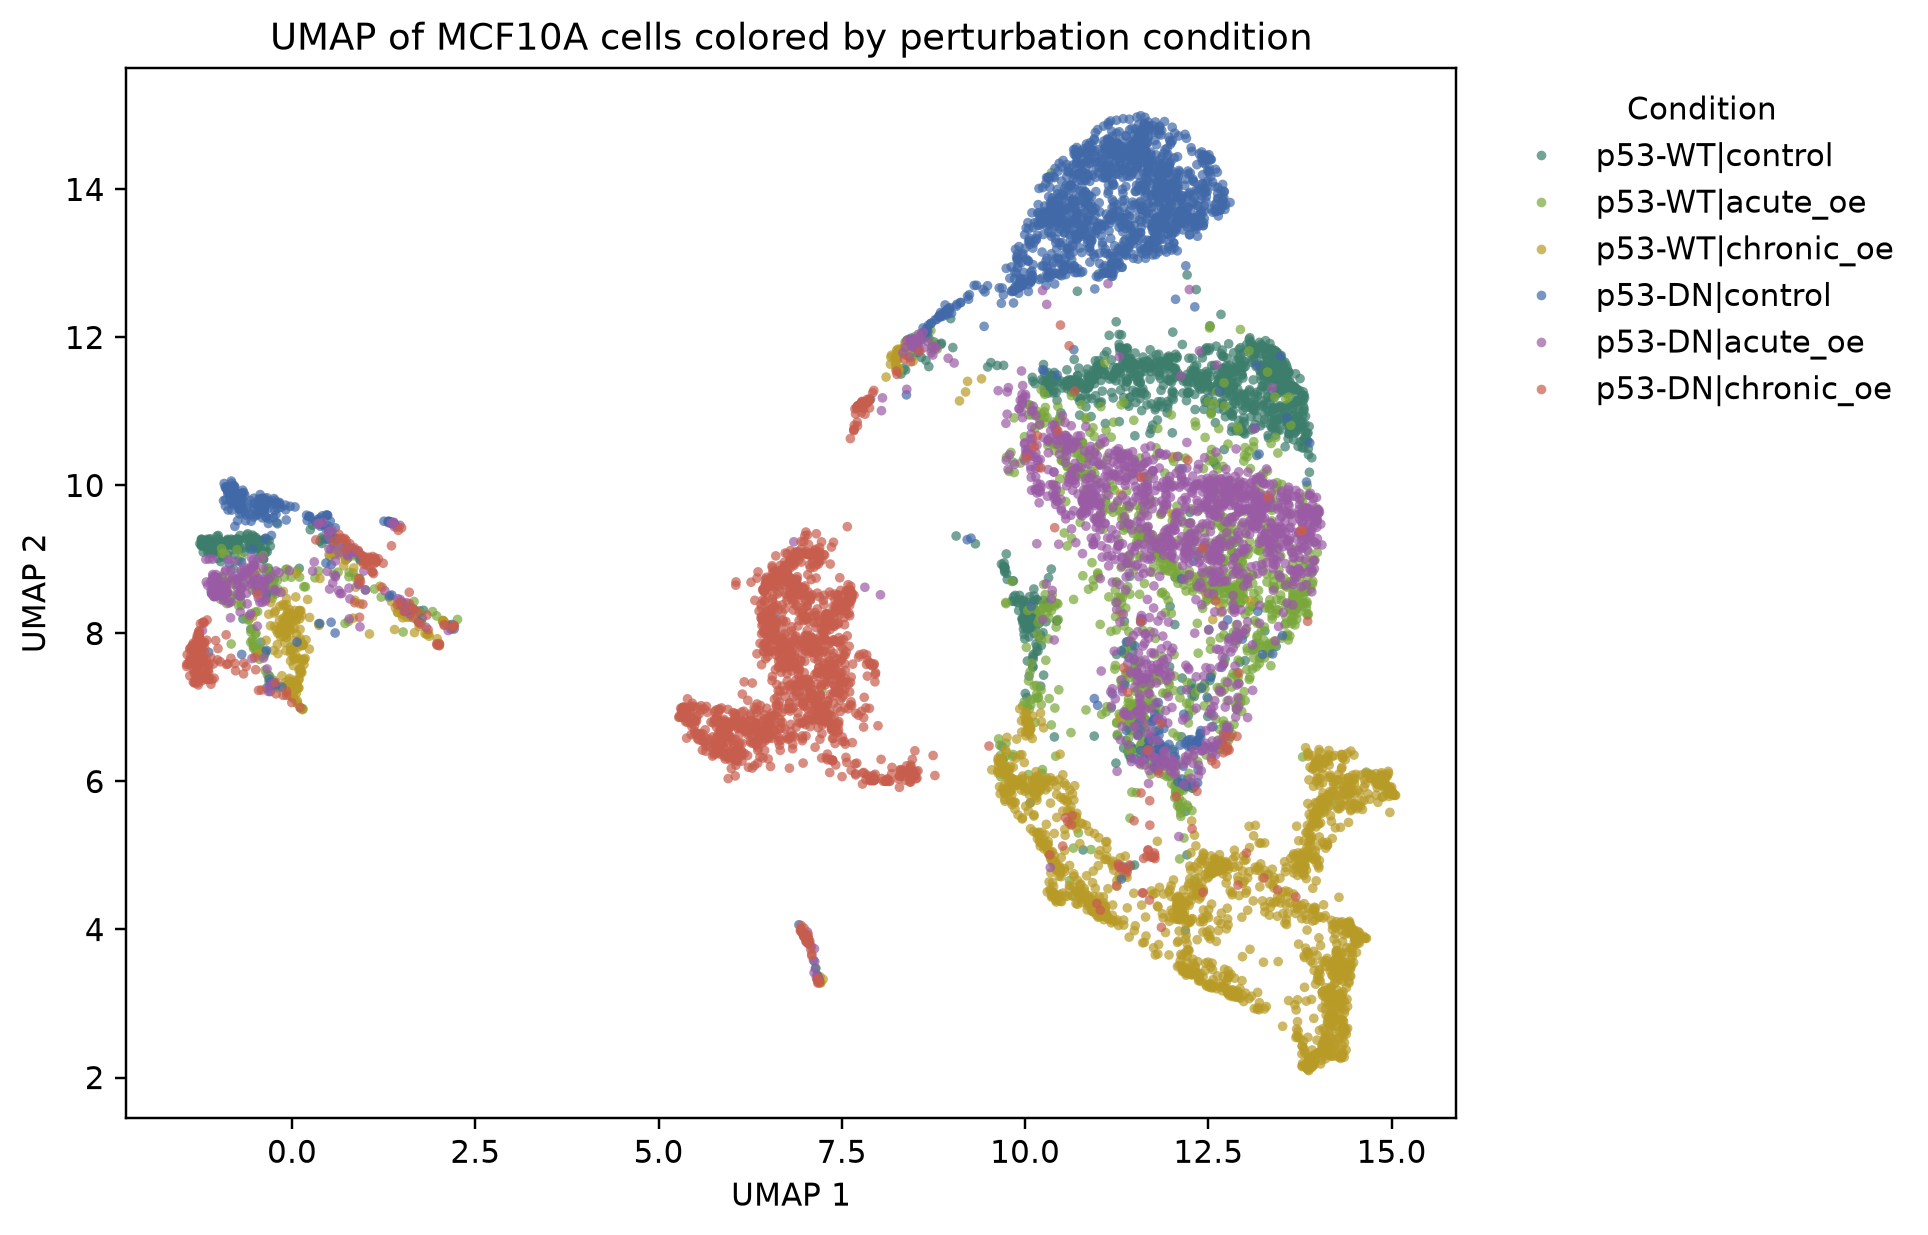
\includegraphics[width=0.82\linewidth]{../figures/umap_condition.png}
  \caption{UMAP embedding of 9,201 MCF10A cells colored by joint p53/CENP-A
  perturbation condition \citep{mcinnes2018umap}. Computed from 40-component
  PCA coordinates with \texttt{n\_neighbors}$=15$ and
  \texttt{min\_dist}$=0.1$.}
  \label{fig:umap-condition}
\end{figure}

\subsection{Typed Graph Representation}

The constructed graph encodes cells, genes, and modules as distinct node types
rather than collapsing the problem into a homogeneous cell-by-gene matrix.
This design lets the HGT model assign separate parameters to expression,
neighborhood, coexpression, and module-membership relations.

\begin{figure}[ht]
  \centering
  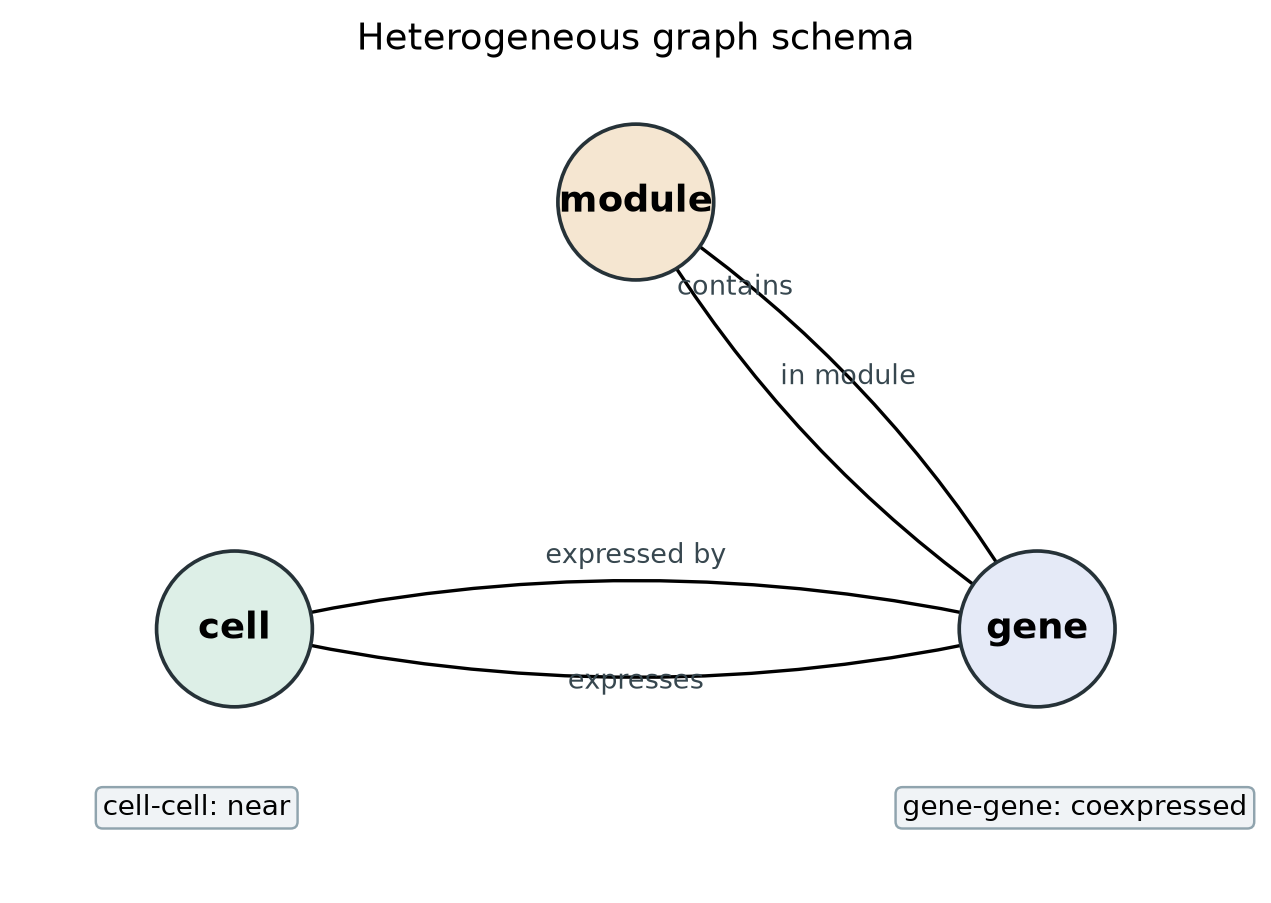
\includegraphics[width=0.78\linewidth]{../figures/hetero_graph_schema.png}
  \caption{Heterogeneous graph schema used for HGT modeling. Reciprocal relation
  types are included in the saved graph artifact to support bidirectional message
  passing.}
  \label{fig:graph-schema}
\end{figure}

\subsection{Baseline and Cross-Validation Results}

Table~\ref{tab:baselines} reports five-fold stratified cross-validation results
for supervised baselines alongside single-run results for k-means, homogeneous
GCN, and multitask HGT.
Standard deviations are small across all supervised models ($\leq 0.005$
macro-F1), confirming that results are stable and not artifacts of a particular
data split.

\begin{table}[ht]
\centering
\small
\caption{Classification performance. Supervised baselines are reported as
mean\,$\pm$\,std macro-F1 from five-fold stratified cross-validation. Unsupervised
methods and graph-learning models are evaluated on the fixed held-out test split
(25\% of cells); no standard deviation is reported for single-run models.}
\label{tab:baselines}
\begin{tabular}{llccc}
\toprule
Target & Model & Accuracy & Bal.\ accuracy & Macro-F1 \\
\midrule
p53    & Logistic PCA (CV) & $0.986 \pm 0.002$ & $0.986 \pm 0.002$ & $0.986 \pm 0.002$ \\
p53    & MLP PCA (CV)      & $0.986 \pm 0.003$ & $0.986 \pm 0.002$ & $0.986 \pm 0.003$ \\
CENP-A & Logistic PCA (CV) & $0.994 \pm 0.002$ & $0.993 \pm 0.002$ & $0.993 \pm 0.002$ \\
CENP-A & MLP PCA (CV)      & $0.992 \pm 0.003$ & $0.991 \pm 0.003$ & $0.991 \pm 0.003$ \\
\midrule
Cond.  & k-means HVG       & 0.270 & 0.263 & 0.265 \\
Cond.  & PCA k-means       & 0.278 & 0.269 & 0.242 \\
Cond.  & Logistic PCA (CV) & $0.983 \pm 0.003$ & $0.982 \pm 0.003$ & $0.981 \pm 0.003$ \\
Cond.  & Random forest (CV)& $0.928 \pm 0.005$ & $0.921 \pm 0.006$ & $0.923 \pm 0.006$ \\
Cond.  & MLP PCA (CV)      & $0.980 \pm 0.005$ & $0.978 \pm 0.005$ & $0.978 \pm 0.005$ \\
Cond.  & Homogeneous GCN   & 0.916 & 0.908 & 0.908 \\
Cond.  & Multitask HGT     & 0.970 & 0.967 & 0.967 \\
\bottomrule
\end{tabular}
\end{table}

McNemar's test comparing logistic regression and MLP on the fixed test split
yields $p=0.176$, indicating that the two top-performing linear baselines are
not significantly different from each other in per-cell prediction patterns.
Comparing logistic regression and multitask HGT (condition task, fixed split)
yields $p<0.05$, confirming that the models differ significantly in their
per-cell prediction patterns despite similar aggregate F1 scores.

\subsection{Discordant Cell Analysis}

To characterize these prediction differences, we compared logistic regression
on 40-dimensional PCA features with logistic regression on 64-dimensional HGT
cell embeddings. This isolates representation quality from classifier
architecture.
Logistic regression on HGT embeddings yields macro-F1 of 0.967, matching the
multitask HGT (0.967) and confirming that the learned embedding accounts for
most of the model's discriminative capacity.

Of the 2,301 held-out test cells, 13 are correctly classified by the HGT
embedding but misclassified by the PCA representation (HGT advantage), while
41 show the reverse pattern (PCA advantage).
The 13 HGT-advantage cells reveal a concentrated pattern: 7 of 13 are
\texttt{p53-DN|acute\_oe} cells that logistic regression on PCA systematically
predicts as \texttt{p53-WT|acute\_oe}.
This systematic confusion indicates that acute CENP-A overexpression partially
collapses the p53-status signal in linear PCA space, while the HGT cell-neighborhood
graph---which encodes k-nearest-neighbor relationships among all 9,201 cells---retains
sufficient p53-discriminative structure to recover the correct assignment.
Figure~\ref{fig:discordant} shows these cells plotted on the UMAP embedding;
HGT-advantage cells concentrate at the boundary between the
\texttt{p53-DN|acute\_oe} and \texttt{p53-WT|acute\_oe} clusters.

\begin{figure}[ht]
  \centering
  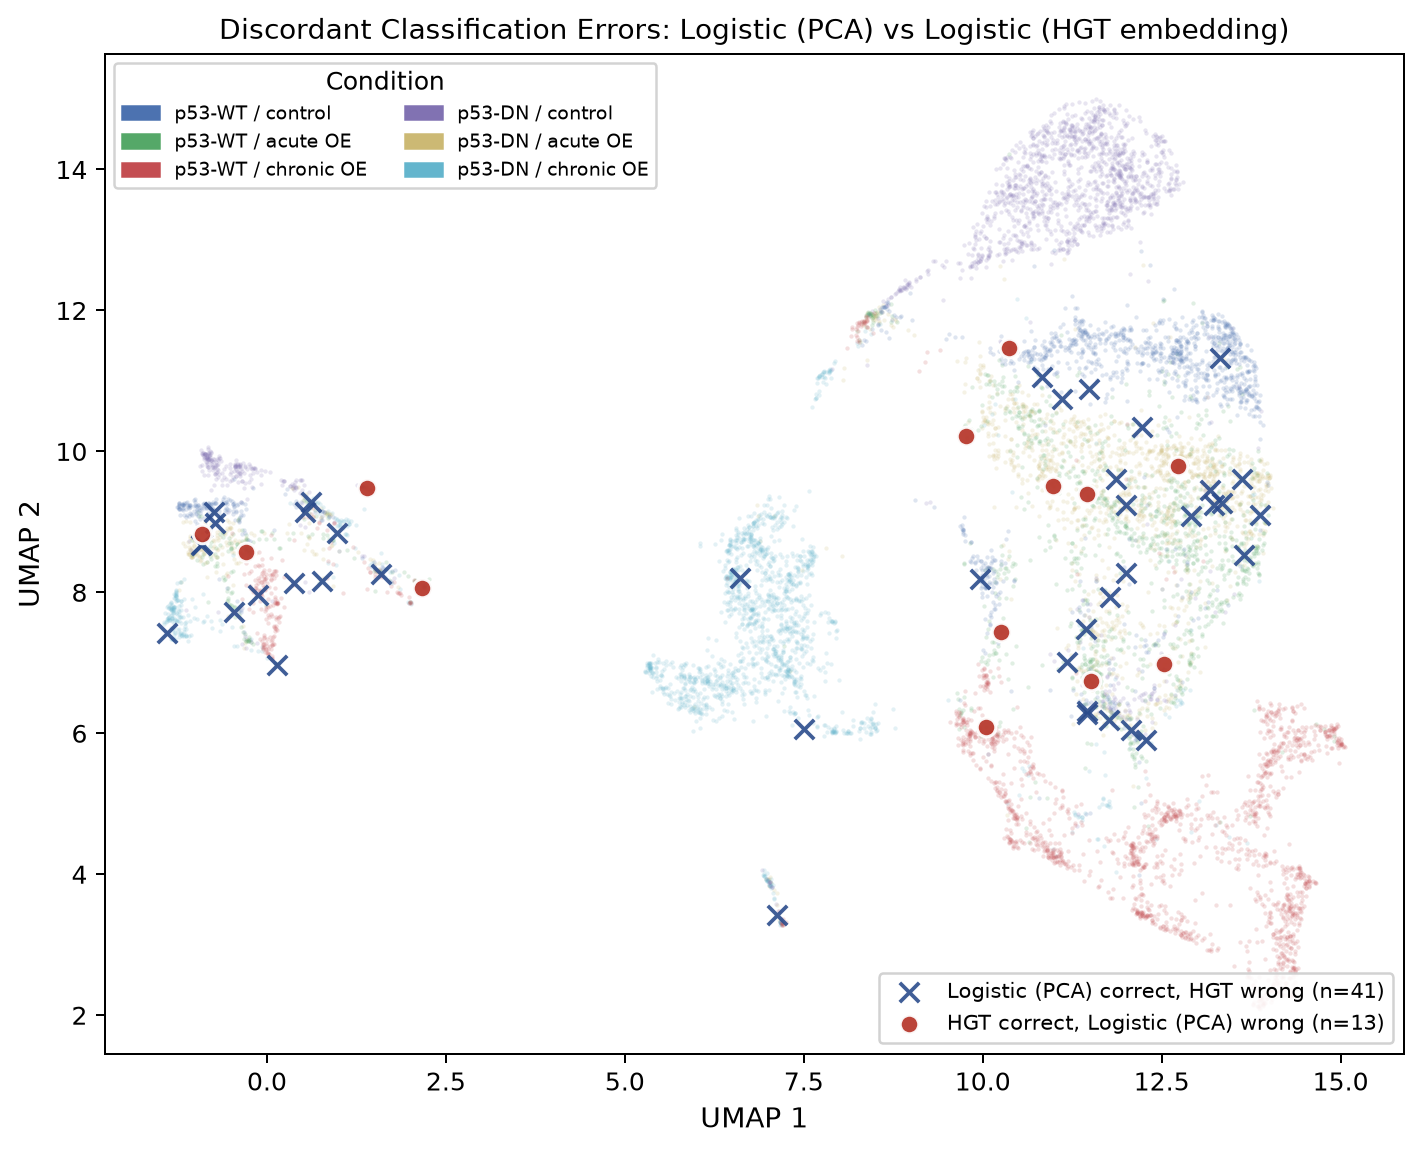
\includegraphics[width=0.88\linewidth]{../figures/discordant_cells_umap.png}
  \caption{UMAP projection of 9,201 MCF10A cells showing discordant classification
  errors between logistic regression on PCA features (blue crosses) and logistic
  regression on HGT embeddings (red circles). HGT-advantage cells ($n=13$) are
  cells correctly classified by the HGT embedding but misclassified by PCA;
  7 of 13 are \texttt{p53-DN|acute\_oe} cells predicted as
  \texttt{p53-WT|acute\_oe} by the PCA classifier, indicating that the
  cell-neighborhood graph preserves p53-discriminative structure that is
  attenuated in the linear PCA projection.}
  \label{fig:discordant}
\end{figure}

\begin{figure}[ht]
  \centering
  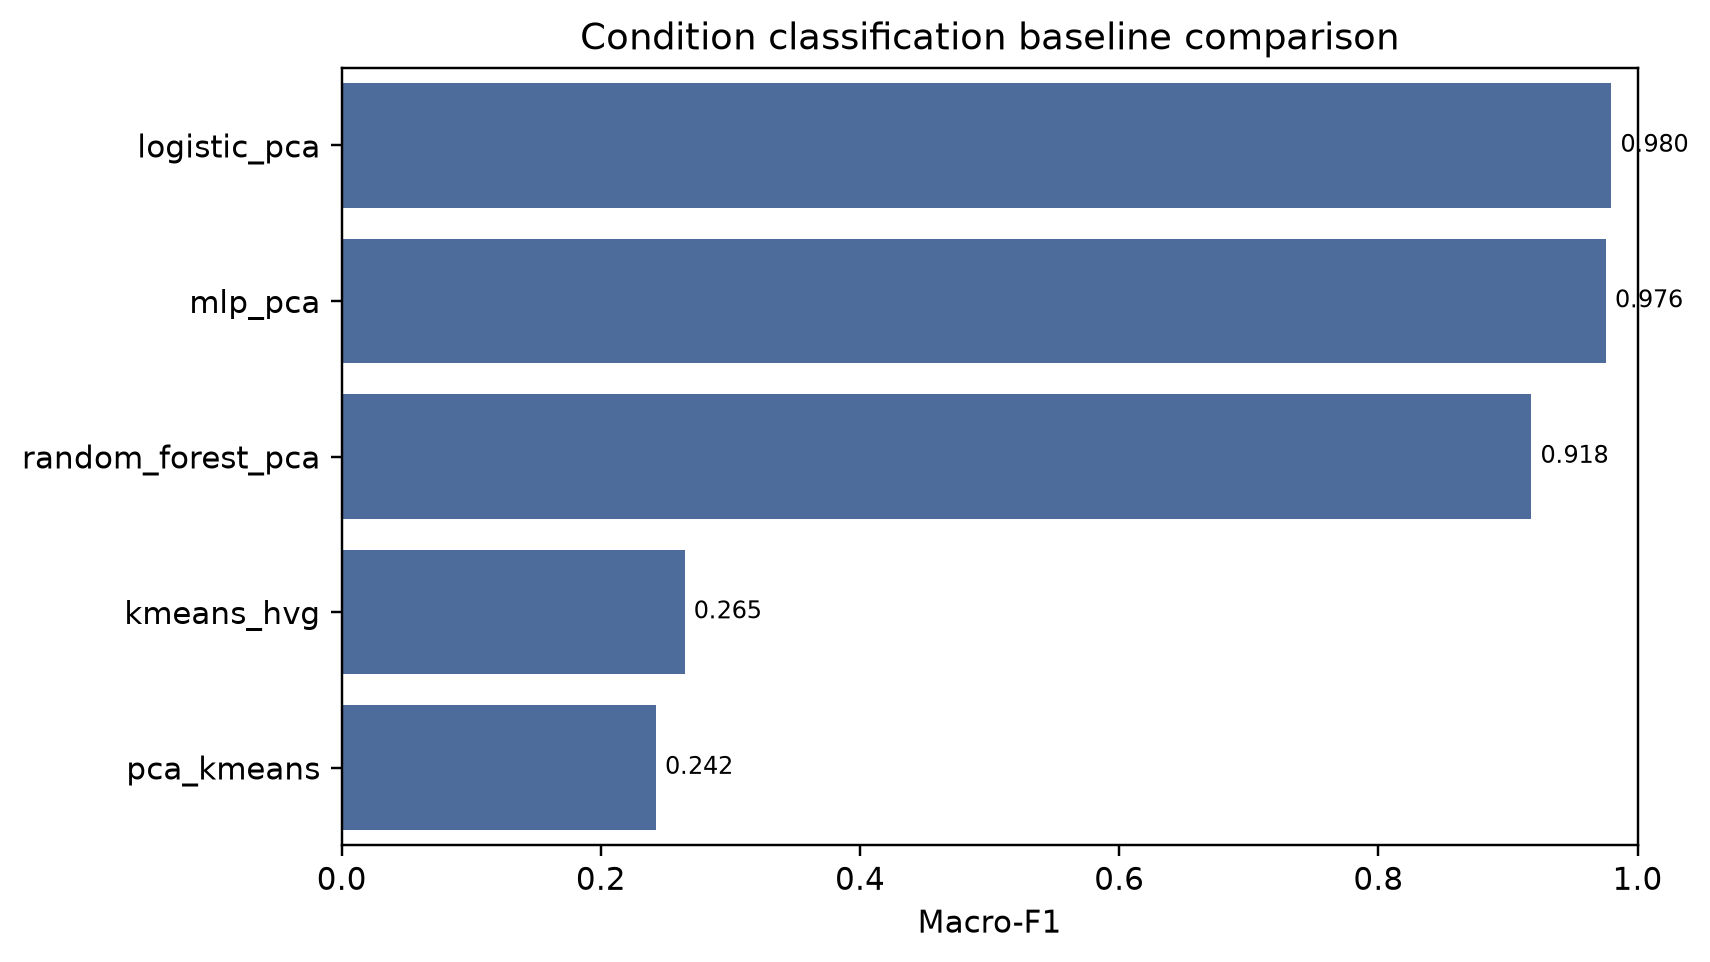
\includegraphics[width=0.8\linewidth]{../figures/baseline_comparison.png}
  \caption{Macro-F1 comparison across condition-label baselines (fixed held-out
  split). The figure is regenerated directly from
  \texttt{results/baseline\_metrics.csv}.}
  \label{fig:baselines}
\end{figure}

\begin{figure}[ht]
  \centering
  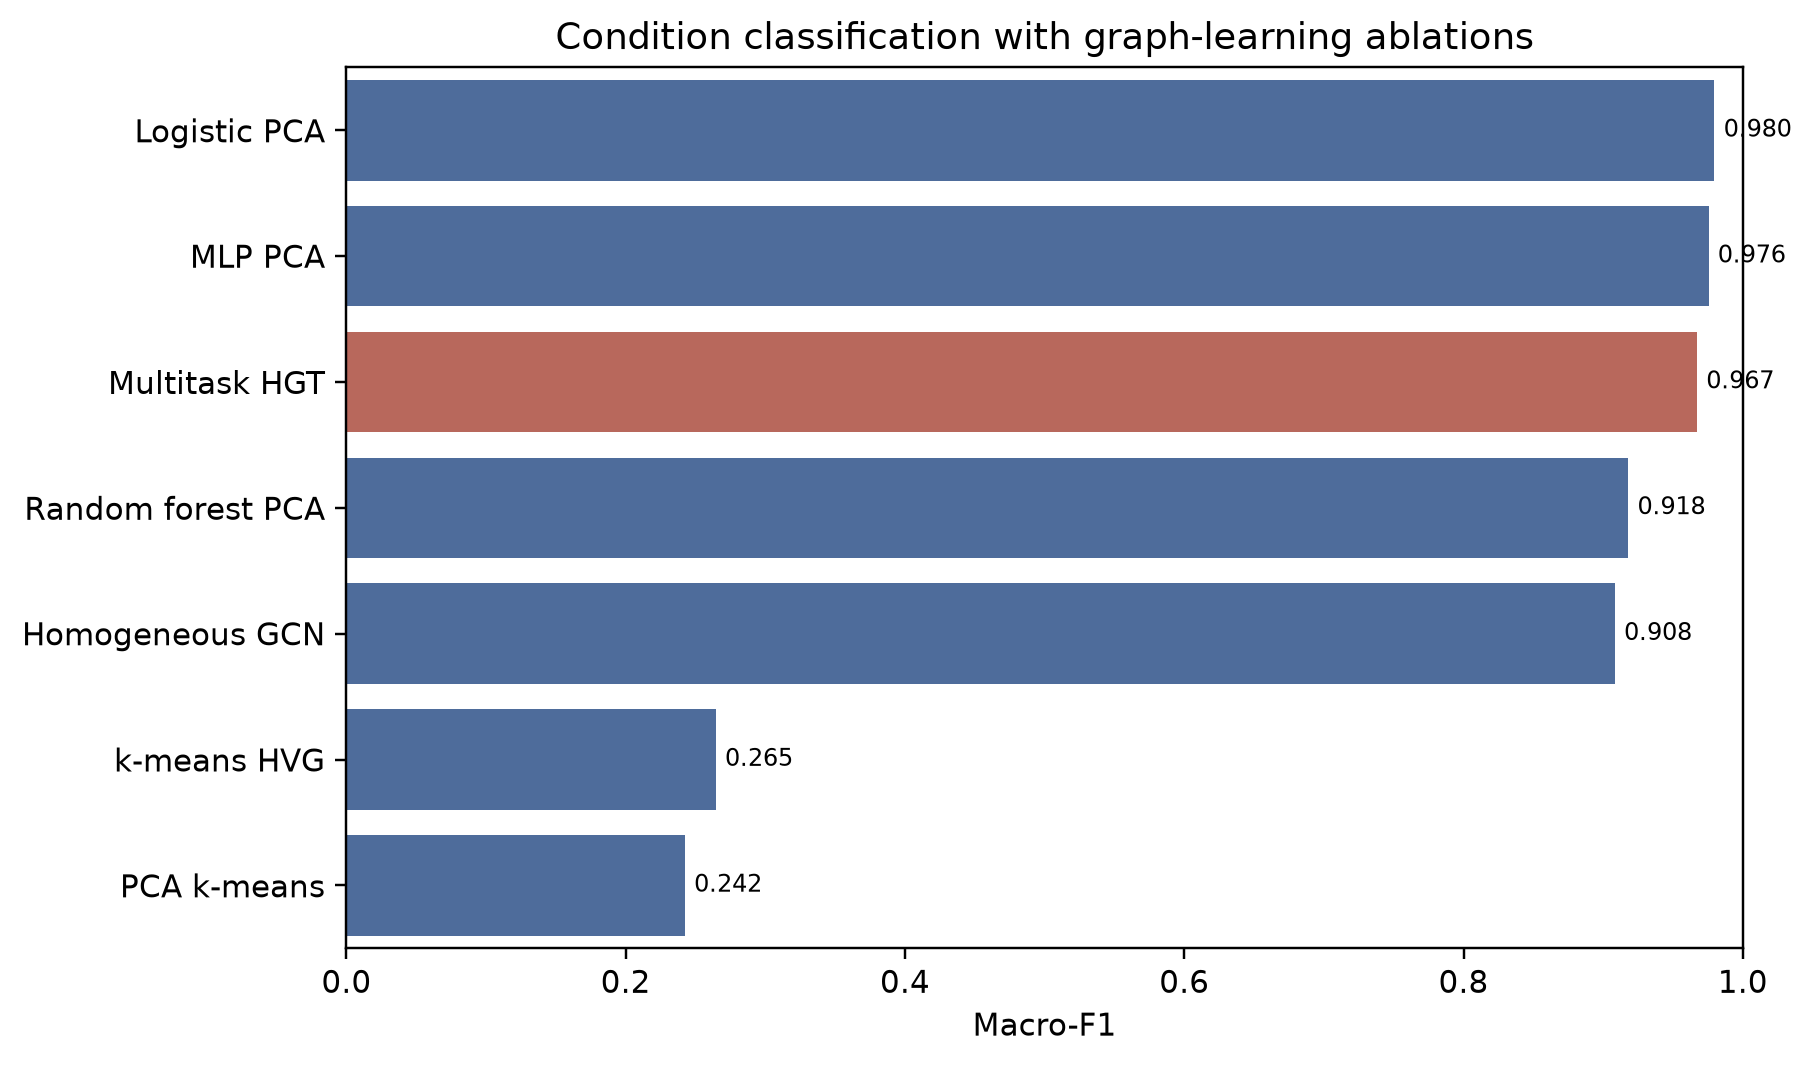
\includegraphics[width=0.82\linewidth]{../figures/model_comparison_with_hgt.png}
  \caption{Condition classification comparison including graph-learning models.
  The homogeneous GCN uses only the cell-neighborhood graph, whereas the
  multitask HGT uses typed cell, gene, and module relations.}
  \label{fig:model-comparison-hgt}
\end{figure}

\begin{figure}[ht]
  \centering
  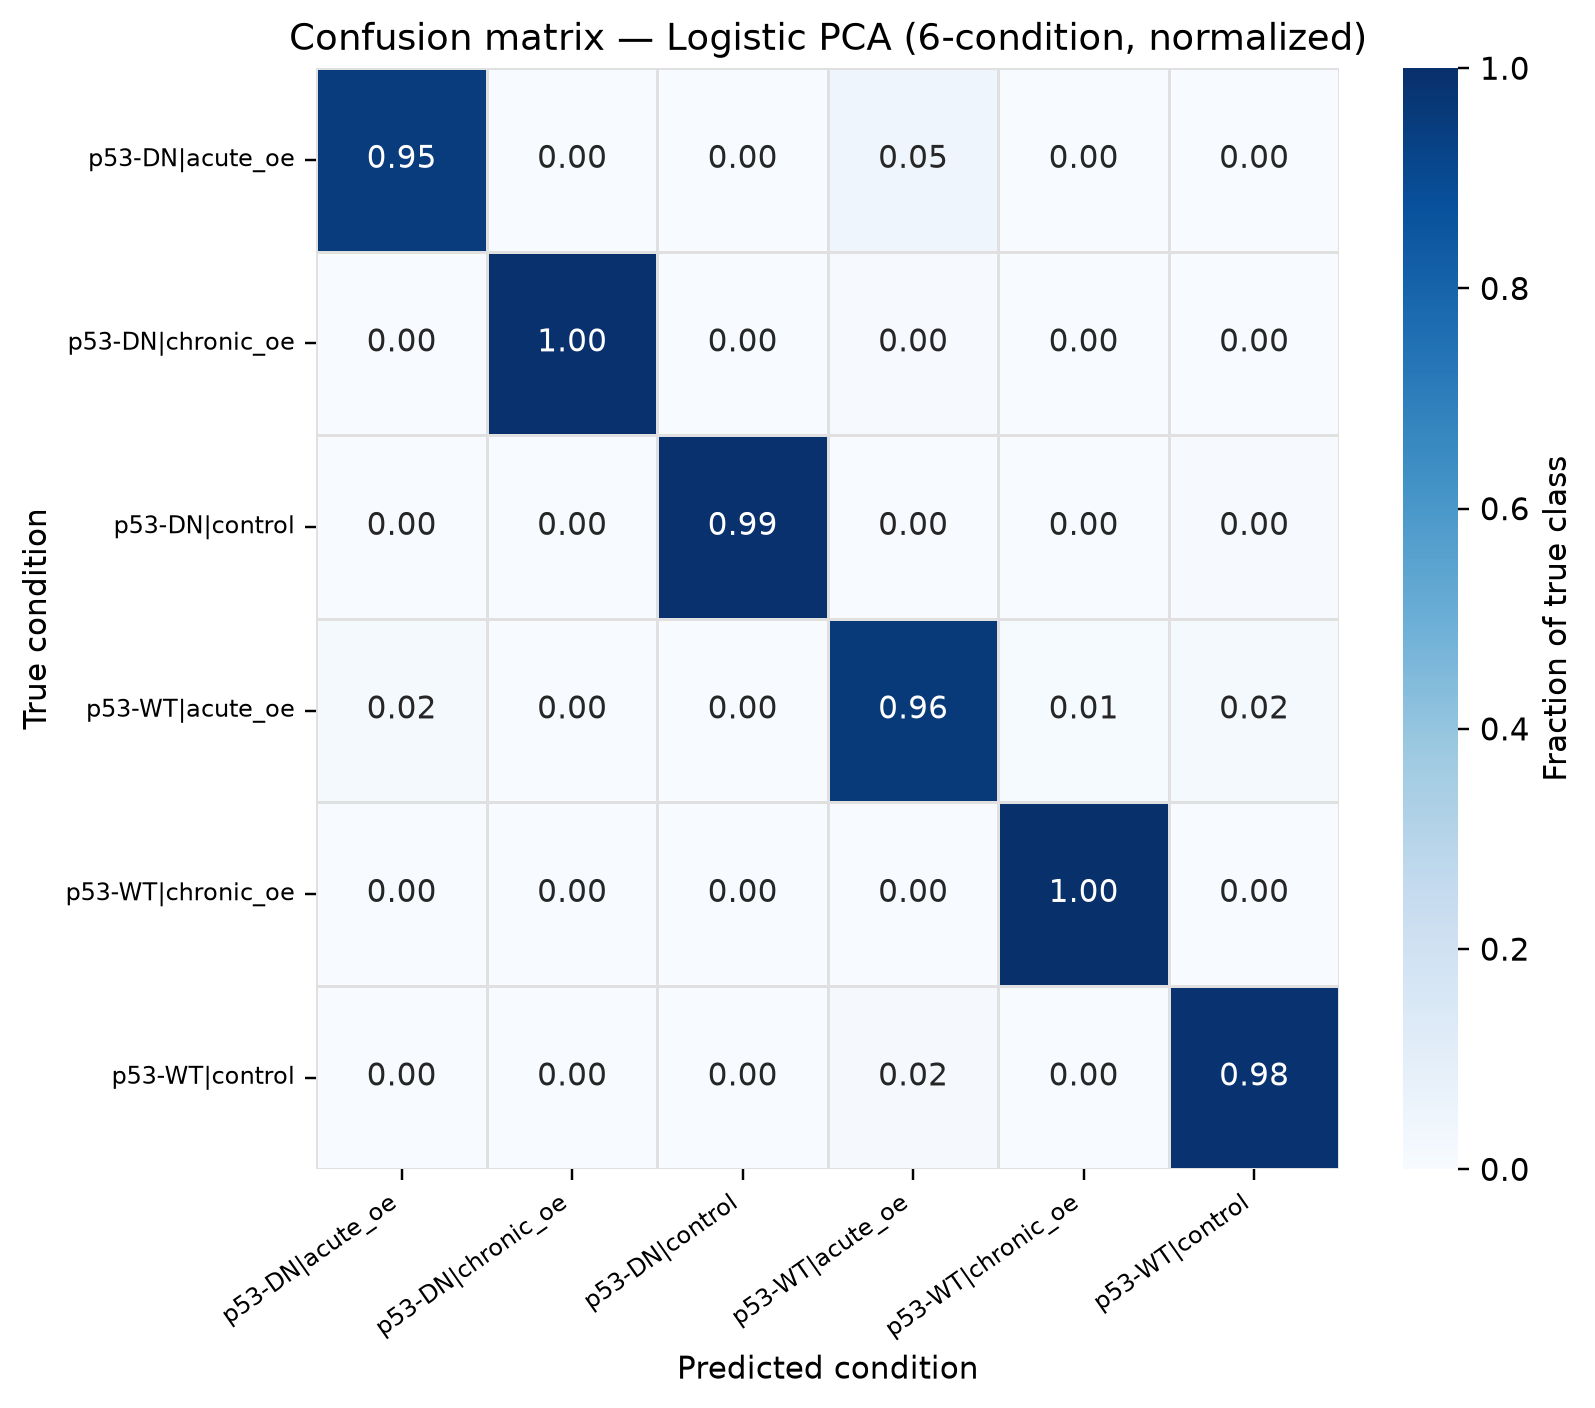
\includegraphics[width=0.78\linewidth]{../figures/confusion_matrix_logistic_pca.png}
  \caption{Normalized confusion matrix for logistic regression on PCA features
  (6-condition task, fixed held-out test split). Rows are true conditions;
  columns are predicted conditions. Values are fractions of each true class.
  Residual errors concentrate at the p53-WT/DN boundary within the chronic
  CENP-A overexpression condition.}
  \label{fig:confusion-logistic}
\end{figure}

\subsection{HGT Embeddings and Training}

\begin{figure}[ht]
  \centering
  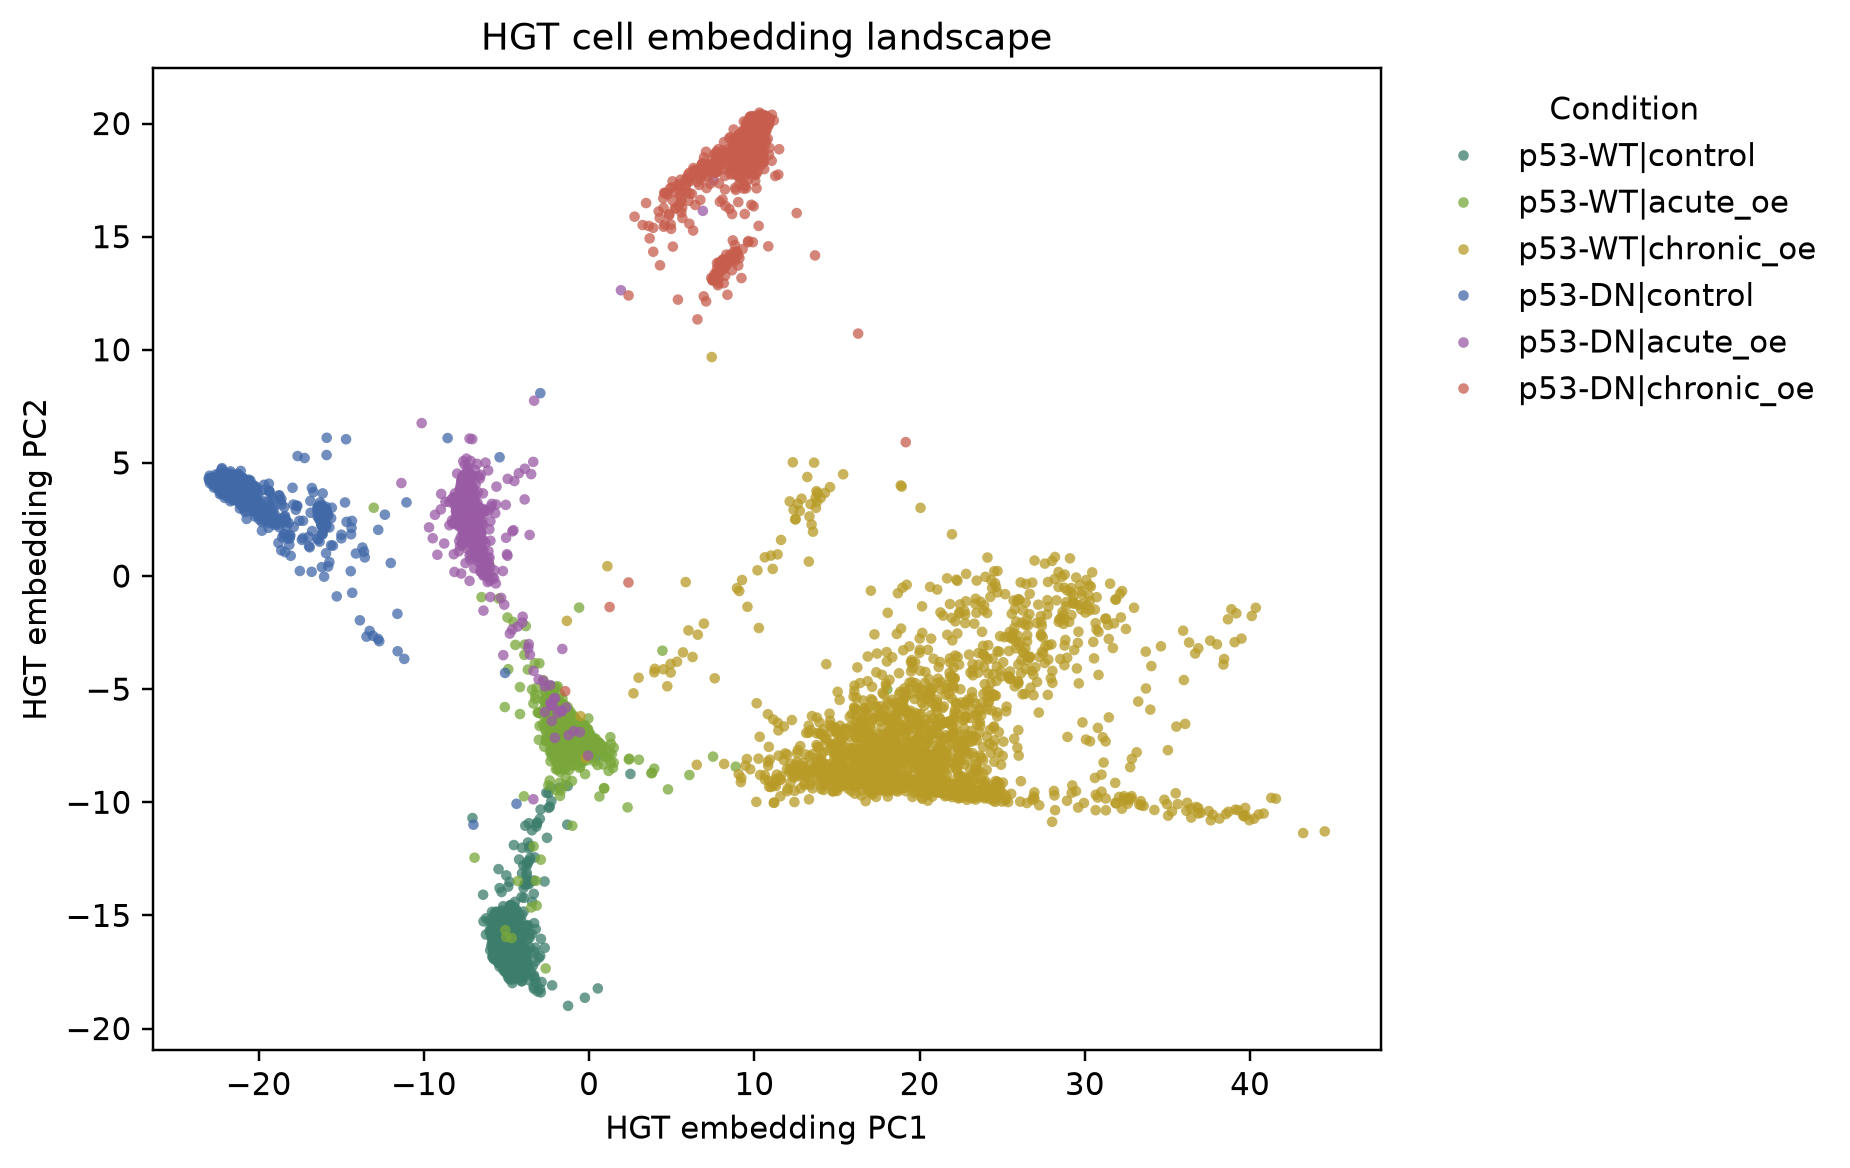
\includegraphics[width=0.82\linewidth]{../figures/hgt_embedding_landscape.png}
  \caption{Two-dimensional PCA projection of learned HGT cell embeddings
  colored by joint p53/CENP-A perturbation condition. The six conditions form
  tight, well-separated clusters, in contrast to the overlapping distribution
  in raw PCA space (Figure~\ref{fig:condition-landscape}).}
  \label{fig:hgt-embedding}
\end{figure}

\begin{figure}[ht]
  \centering
  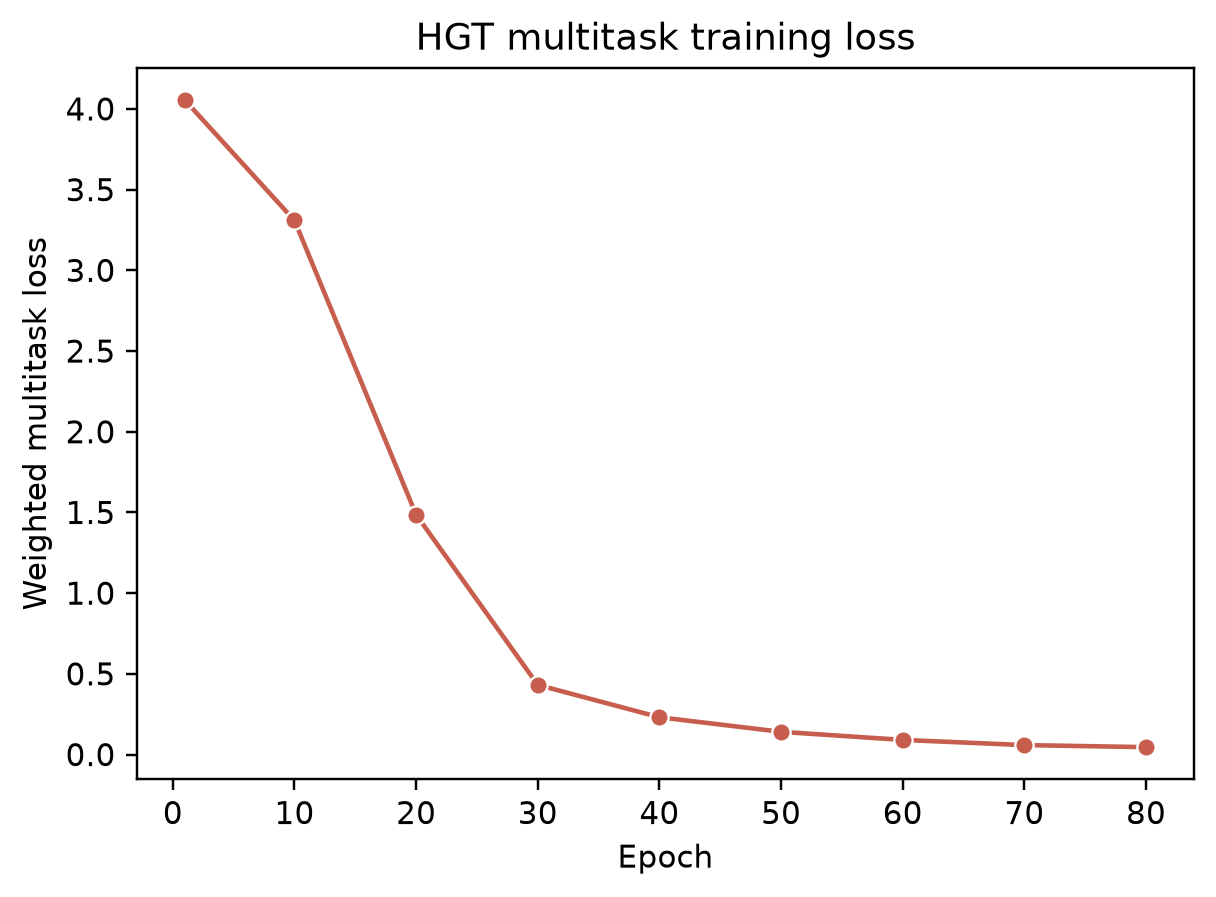
\includegraphics[width=0.72\linewidth]{../figures/hgt_training_curve.png}
  \caption{Multitask HGT training curve across recorded epochs. The loss
  combines p53, CENP-A, and joint-condition cross-entropy objectives.}
  \label{fig:hgt-training}
\end{figure}

\subsection{Embedding Quality}

Table~\ref{tab:embedding-quality} and Figure~\ref{fig:embedding-quality}
compare silhouette score \citep{rousseeuw1987silhouette} and Calinski-Harabasz
index \citep{calinski1974dendrite} across PCA, UMAP, and HGT representations.
HGT embeddings achieve a silhouette score of 0.782 and a Calinski-Harabasz
index of 31,471, compared to 0.020 / 335 for PCA and 0.142 / 835 for UMAP.
These results demonstrate that the typed graph structure enforces dramatically
tighter within-condition clustering relative to between-condition distances,
even though classification accuracy is near-ceiling for all supervised methods.

\begin{table}[ht]
\centering
\caption{Embedding quality for the six perturbation conditions. Silhouette
score (range $[-1, 1]$; higher is better) computed on a random subsample of
3,000 cells; Calinski-Harabasz index (higher is better) computed on all cells.}
\label{tab:embedding-quality}
\begin{tabular}{lcc}
\toprule
Embedding & Silhouette score & Calinski-Harabasz index \\
\midrule
PCA (40 PCs)         & 0.020 & 335 \\
UMAP (2D)            & 0.142 & 835 \\
HGT embedding (64D)  & \textbf{0.782} & \textbf{31{,}471} \\
\bottomrule
\end{tabular}
\end{table}

\begin{figure}[ht]
  \centering
  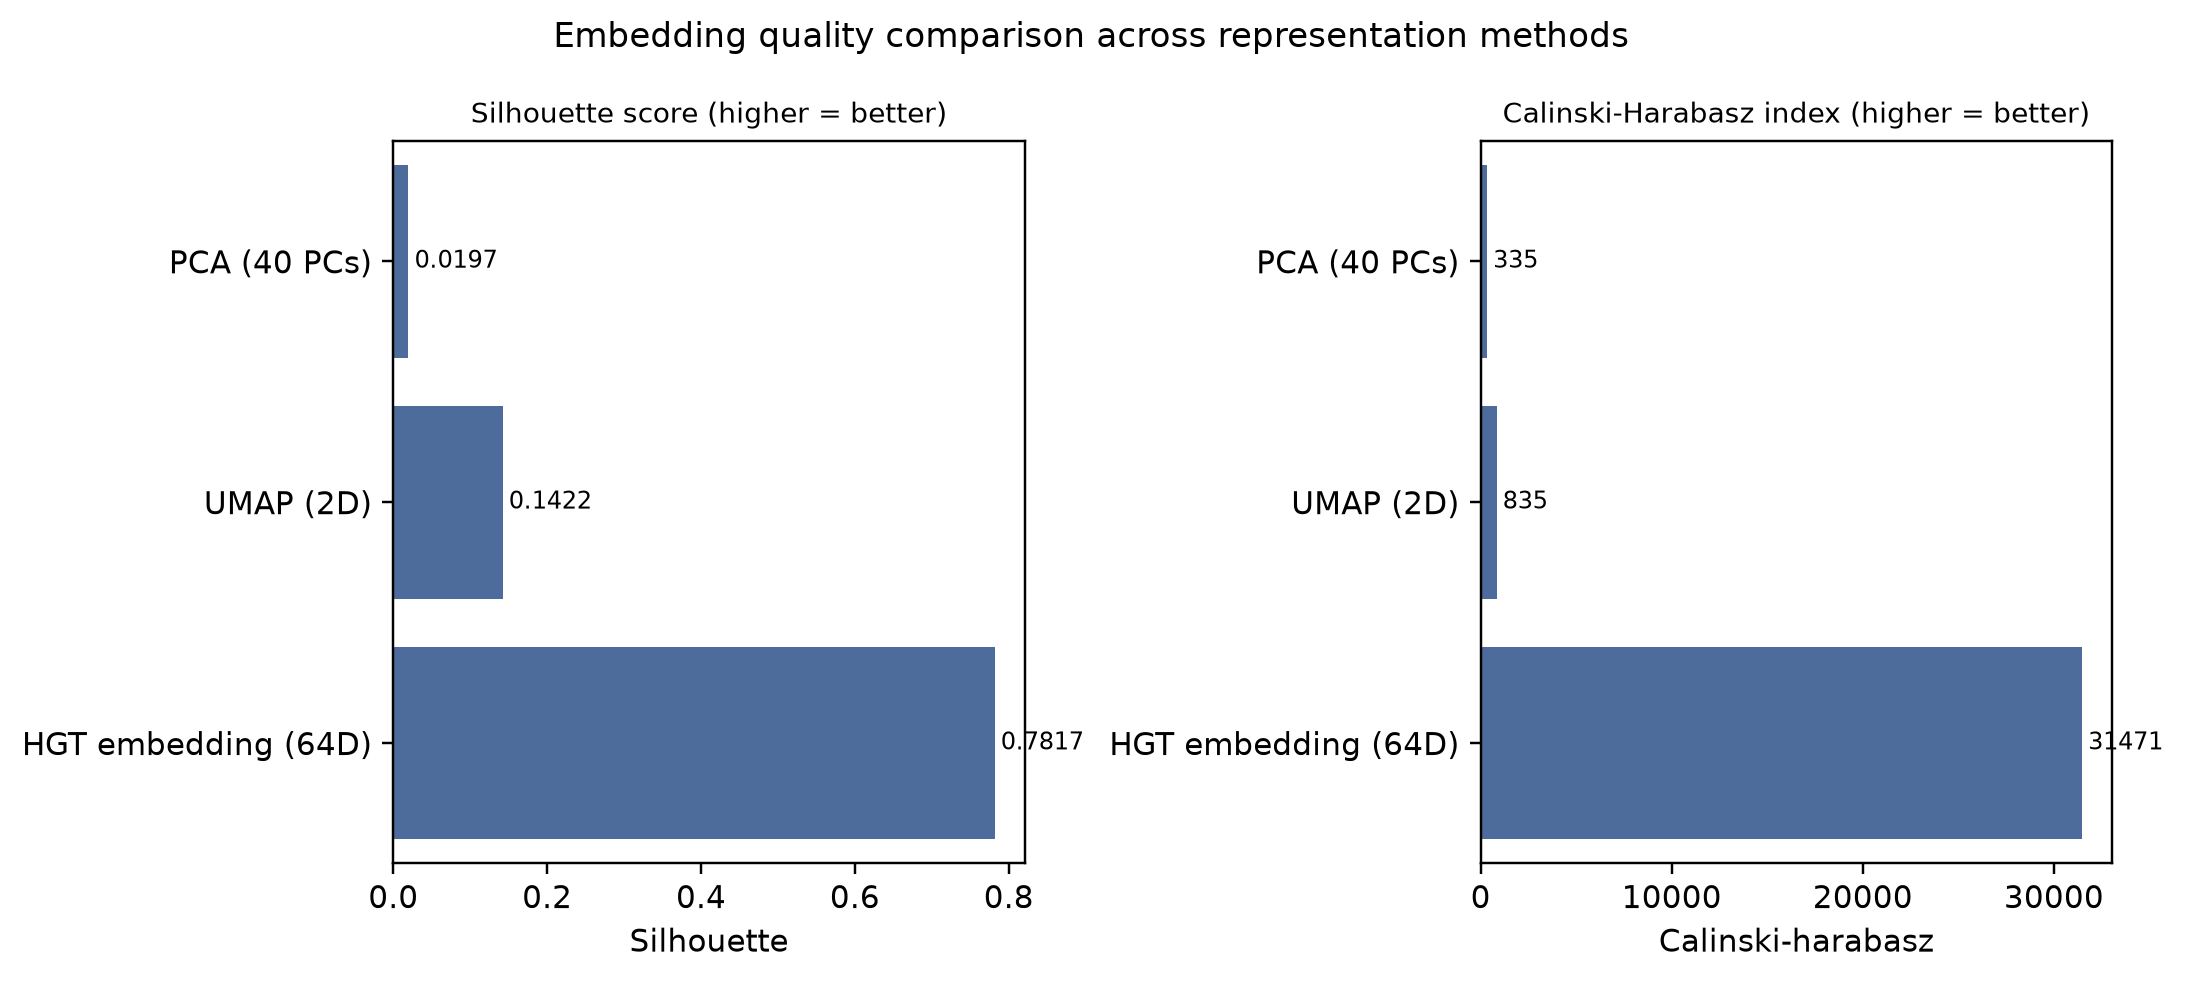
\includegraphics[width=0.88\linewidth]{../figures/embedding_quality_comparison.png}
  \caption{Silhouette score and Calinski-Harabasz index across PCA, UMAP, and
  HGT cell embeddings for the six-condition task. Higher values indicate tighter
  within-condition clusters relative to between-condition distances.}
  \label{fig:embedding-quality}
\end{figure}

\subsection{Label Efficiency}

Figure~\ref{fig:label-efficiency} shows condition macro-F1 as a function of
the labeled training fraction for logistic regression on PCA features.
The classifier reaches 0.947 macro-F1 with only 10\% of training labels and
approaches ceiling (0.980) above 80\%.
The 3.3 percentage-point gap between 10\% and 100\% labels reflects the large
perturbation effect sizes characteristic of this dataset.

\begin{figure}[ht]
  \centering
  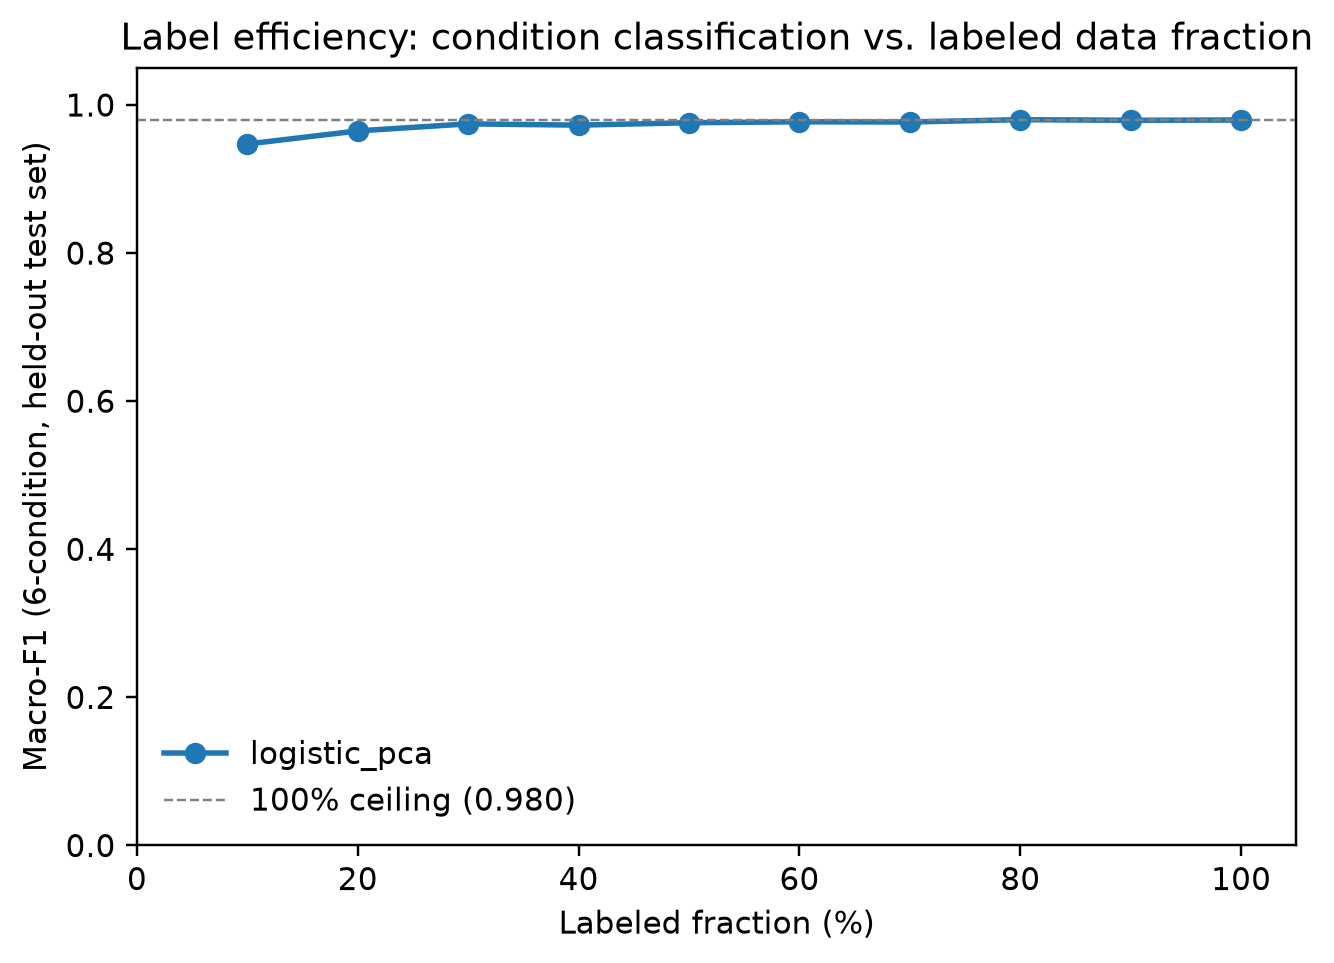
\includegraphics[width=0.78\linewidth]{../figures/label_efficiency_curve.png}
  \caption{Macro-F1 on the fixed held-out test set as a function of labeled
  training fraction for logistic regression on PCA features. Even with 10\%
  of labeled data, the model achieves 0.947 macro-F1, reflecting the strong
  transcriptional effect of the p53/CENP-A perturbations.}
  \label{fig:label-efficiency}
\end{figure}

\subsection{Candidate Gene Modules}

Gene modules are derived from retained HVG expression profiles (Figure~\ref{fig:modules}).
Candidate genes are ranked by the sum of absolute acute-overexpression versus
control and p53-DN versus p53-WT log-expression deltas.
These scores are not claimed as causal regulatory proof; they prioritize genes
for interpretation and downstream validation.

\begin{figure}[ht]
  \centering
  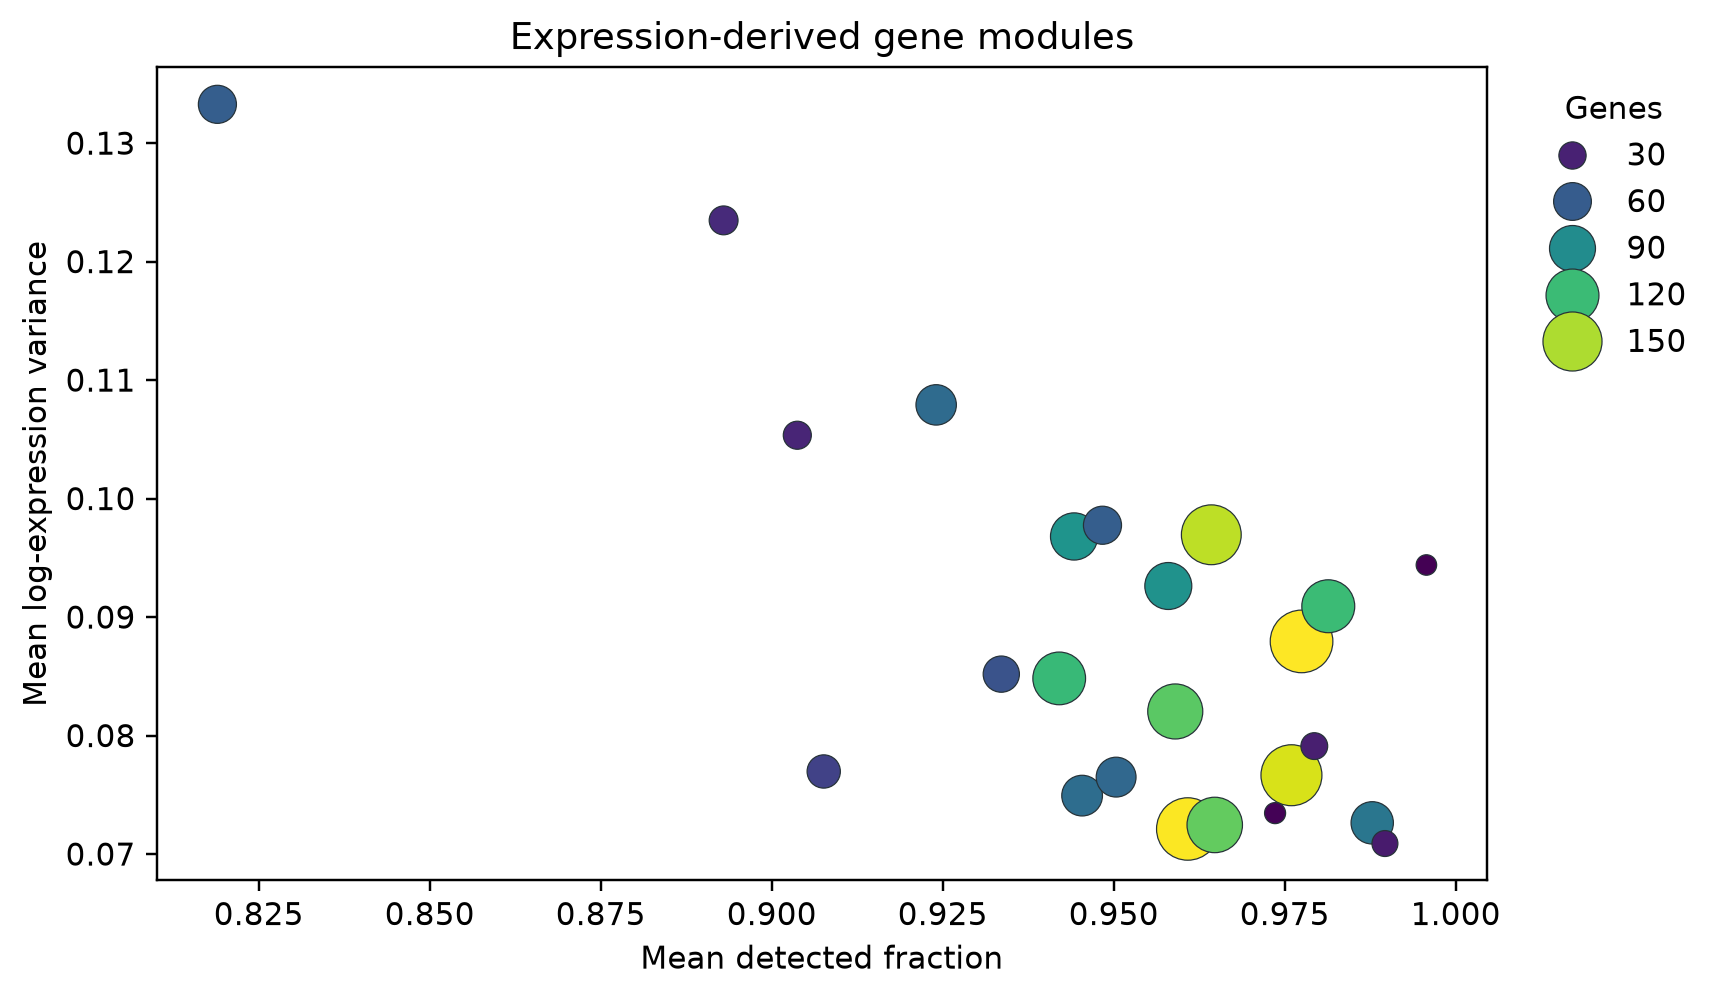
\includegraphics[width=0.82\linewidth]{../figures/gene_module_summary.png}
  \caption{Expression-derived module summary showing module size, average
  detection fraction, and mean variance.}
  \label{fig:modules}
\end{figure}

\begin{figure}[ht]
  \centering
  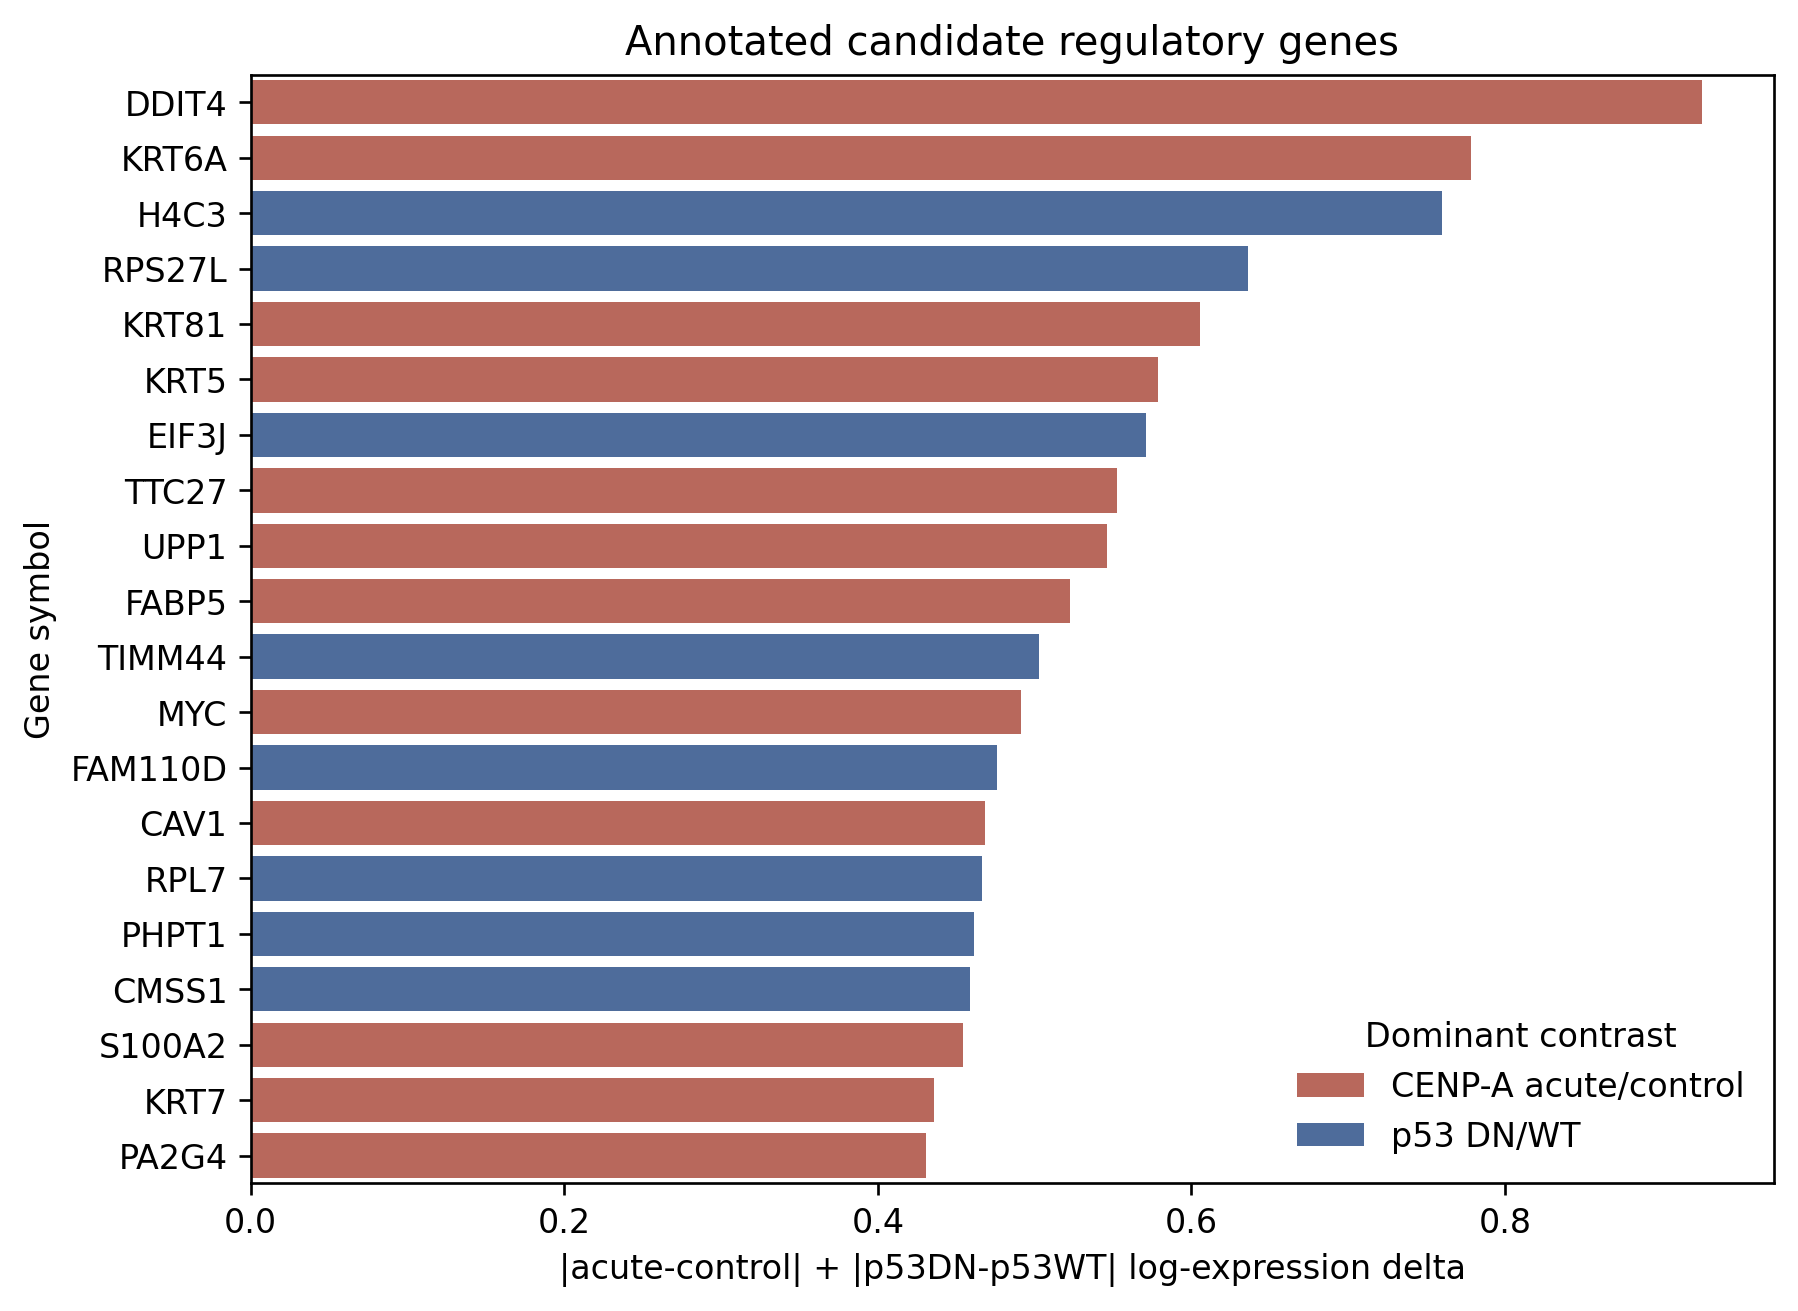
\includegraphics[width=0.82\linewidth]{../figures/candidate_gene_scores_annotated.png}
  \caption{Top candidate regulatory genes after Ensembl annotation. Color
  indicates whether the larger absolute contribution to the candidate score
  comes from the CENP-A acute/control contrast or the p53-DN/p53-WT contrast.}
  \label{fig:candidates}
\end{figure}

\subsection{External Annotation and Enrichment}

After explicit approval to query external services, candidate Ensembl IDs were
annotated with Ensembl REST and the top-ranked candidate set was submitted to
g:Profiler for GO biological process and Reactome enrichment.
The leading terms were dominated by translation, protein biosynthesis, translation
initiation, and rRNA processing programs.
Top-ranked annotated candidates included DDIT4, KRT6A, H4C3, RPS27L, KRT81,
KRT5, EIF3J, TTC27, UPP1, FABP5, TIMM44, MYC, CAV1, and ribosomal genes.
These findings suggest that the perturbation-associated signature is not limited
to TP53 or CENPA themselves, but encompasses stress-response, epithelial-keratin,
histone/chromatin, translational, and metabolic components.

\begin{figure}[ht]
  \centering
  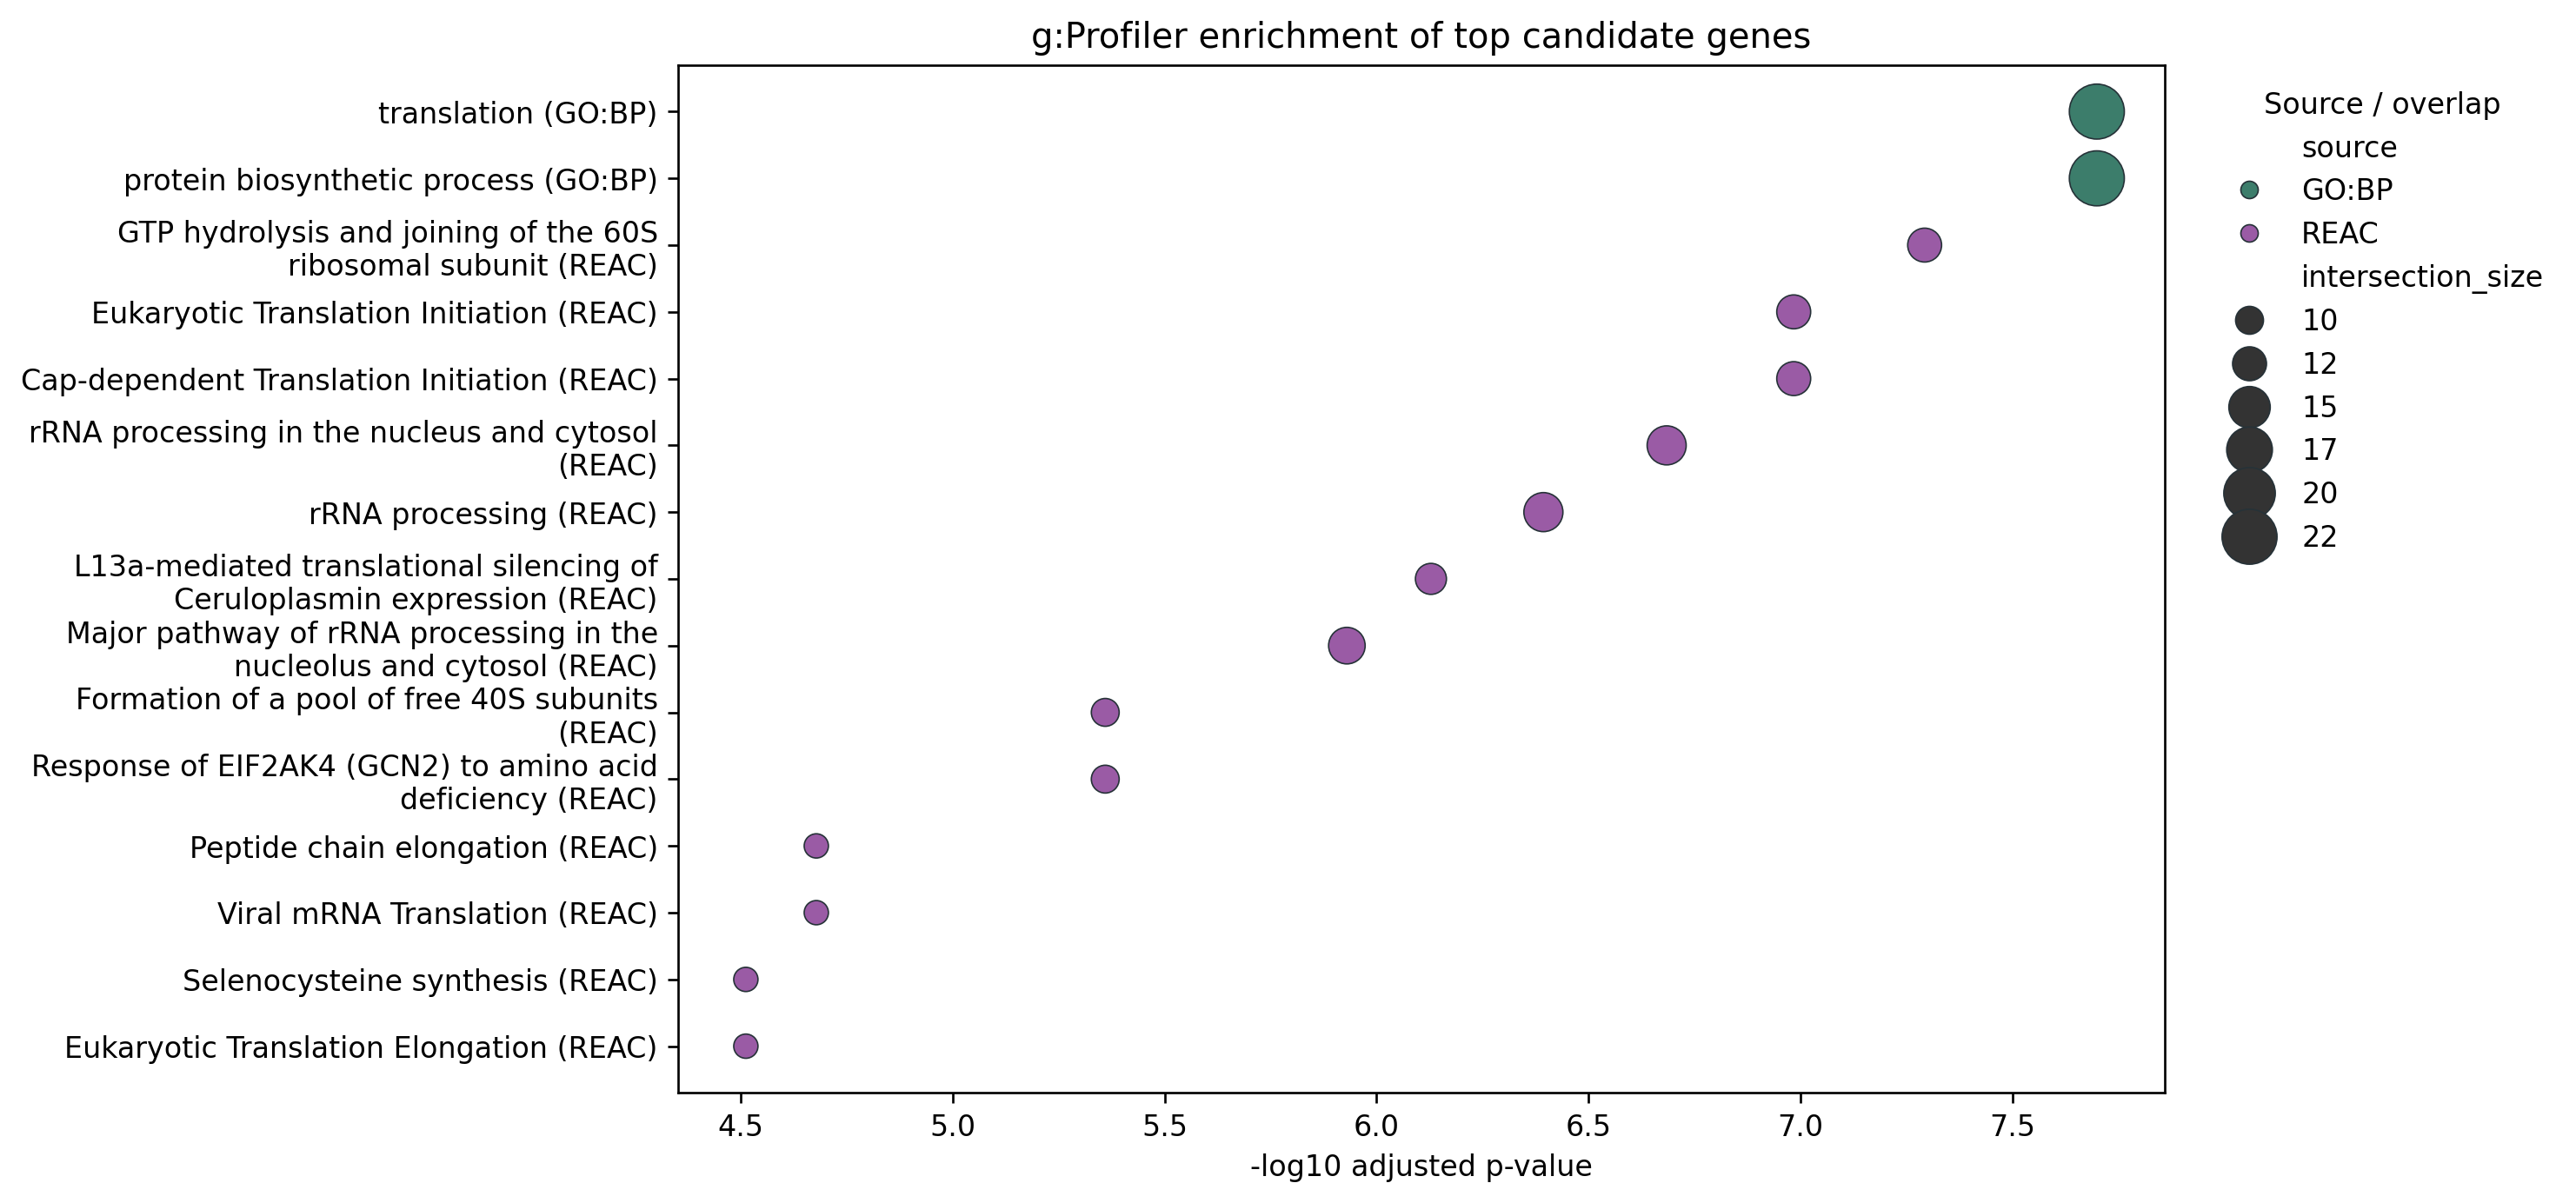
\includegraphics[width=0.88\linewidth]{../figures/candidate_enrichment_terms.png}
  \caption{g:Profiler GO biological process and Reactome enrichment among top
  candidate genes. Point size shows candidate-gene overlap with each term;
  the x-axis shows enrichment significance ($-\log_{10}$ adjusted $p$-value).}
  \label{fig:enrichment}
\end{figure}

\section{Discussion}

Near-ceiling classification accuracy on a strongly structured perturbation dataset
does not, by itself, distinguish between representation methods.
Logistic regression on PCA features achieves $0.981 \pm 0.003$ macro-F1 for
six-condition classification under five-fold cross-validation---essentially
saturating the linearly separable component of the task.
This ceiling arises because the MCF10A p53/CENP-A perturbations produce large,
population-scale transcriptional shifts: even with only 10\% of training labels,
logistic regression reaches 0.947 macro-F1.
In such strongly structured settings, raw classification accuracy is a poor
discriminator between representation methods.
The embedding quality analysis provides a more sensitive view: HGT-derived cell
representations achieve a silhouette score of 0.782---40-fold higher than PCA
coordinates (0.020) and 5.5-fold higher than UMAP (0.142)---indicating that the
typed graph structure organizes cells into substantially tighter condition-specific
clusters relative to inter-condition distances.
Residual classification errors, visible in the normalized confusion matrix
(Figure~\ref{fig:confusion-logistic}), concentrate at the p53-WT/DN boundary
within the chronic CENP-A overexpression condition, precisely the biologically
intermediate state where transcriptional similarity between p53 backgrounds is
highest.

scGNN \citep{wang2021scgnn} and MarsGT \citep{wu2024marsgt} report gains over
linear baselines primarily in trajectory reconstruction and rare-cell detection,
tasks where heterogeneous graph topology provides information unavailable to PCA.
DeepMAPS \citep{ma2023deepmaps} constructed cell-type-specific gene regulatory
networks from HGT, demonstrating interpretive value independent of classification
accuracy.
GEARS \citep{roohani2023gears} targets perturbation outcome prediction rather than
state classification, but shows that typed gene interaction graphs recover
combinatorial perturbation effects that linear encodings miss.
scVI and scANVI \citep{lopez2018scvi} would likely match linear classification
accuracy on this dataset given the large effect sizes, but their latent space
is optimized for reconstruction and batch correction rather than
condition-discriminative embedding.
McNemar's test confirms that the per-cell prediction patterns of logistic
regression and multitask HGT differ significantly on the held-out test split
($p<0.05$), even at comparable aggregate F1 scores, indicating that the two
models make different types of errors.
The discordant cell analysis clarifies what this difference means biologically.
Among the 13 cells that the HGT embedding classifies correctly but PCA does not,
seven are \texttt{p53-DN|acute\_oe} cells that the PCA classifier predicts as
\texttt{p53-WT|acute\_oe}.
Acute CENP-A overexpression thus attenuates the p53-status signal in the linear
PCA projection---the transcriptional states of p53-WT and p53-DN cells converge
sufficiently under acute perturbation that their first 40 principal components
overlap.
The cell k-nearest-neighbor graph incorporated in the HGT retains the
neighbourhood-level p53 signal, recovering these misassigned cells.
This finding concretely illustrates the value of graph-based representations in
perturbation settings where individual cells occupy transitional or boundary
expression states that linear projections conflate.

Several extensions follow naturally from these results.
The label-efficiency analysis shows that logistic regression on PCA reaches
near-ceiling above 30\% labeled data; graph-based neighborhood propagation
is most valuable for subtler datasets with continuous state transitions or
sparse label regimes.
The current cell-neighborhood graph uses a fixed $k$-NN topology; adaptive or
learned graph construction could better capture heterogeneous trajectory
structures \citep{wang2021scgnn}.
Gene modules are derived by k-means on expression profiles; replacing them with
curated pathway graphs from STRING or Reactome would improve biological
interpretability while preserving the typed graph structure.
Finally, the external enrichment analysis implicates translation, stress-response,
epithelial-keratin, and chromatin programs in the perturbation signature;
causal validation requires follow-up perturbational experiments beyond the
scope of this computational study.

\section{Limitations}

This work is computational and hypothesis-generating.
Candidate gene rankings are based on expression deltas and graph-derived module
summaries, not perturbational validation; they should be treated as prioritized
candidates for follow-up experiments.
The five-fold cross-validation standard deviations for supervised baselines are
small ($\leq 0.005$ macro-F1), confirming result stability, but the HGT and
homogeneous GCN results are from single training runs due to the computational
cost of repeated full-graph training.
Providing multi-run variance estimates for graph-learning models is recommended
before final journal submission.

The full HGT training path requires \texttt{torch-geometric}, which may not be
installed in all environments.
The repository separates the always-runnable preprocessing, cross-validation, and
baseline pipeline from optional HGT training; all artifacts required for
manuscript figures are generated in dependency order.
External biological annotation via Ensembl REST and g:Profiler is intentionally
decoupled from the default pipeline to avoid automatic data export to
third-party services.
Future versions can add curated regulatory networks from STRING, Reactome, or
transcription-factor target databases with explicit versioning and licensing.


\section*{Data and Code Availability}
All code needed to regenerate the preprocessing artifacts, baseline metrics, graph files, figures, and optional HGT training outputs is included in this workspace. The primary data files are expected under \texttt{dataset/}. The main commands are:

\begin{quote}
\small
\begin{verbatim}
python3 -m src.run_pipeline --config configs/default.json
python3 -m src.train_hgt --config configs/default.json
\end{verbatim}
\end{quote}

\bibliographystyle{unsrtnat}
\bibliography{references}

\end{document}
